%
%  thesis.tex  2014-01-15  Mark Senn  http://engineering.purdue.edu/~mark
%
%  This is the thesis ``root file''.
%
%  To print the final copy of your thesis put a '%'
%  in front of the \includeonly command and type
%  (from page 71 of _LaTeX User's Guide and Reference Manual_, 2nd edition):
%      latex thesis
%      bibtex thesis
%      latex thesis
%      latex th	esis
%
%  In "Reference:" listings below:
%      KEY  MEANING
%      TM   ``A Manual for the Preparation of Graduate Theses'',
%             seventh revised edition, The Graduate School, 2006.
%             http://www2.itap.purdue.edu/gradschool//Publications/graduate-thesis-manual.pdf
%      PU   ``A Manual for the Preparation of Graduate Theses'',
%           The Graduate School, Purdue University, 1996.
%           http://www2.itap.purdue.edu/gradschool//Publications/graduate-thesis-manual.pdf
%
%  Search for "CHANGE" below and change things as necessary.
%  I recommend putting "%%" before any existing lines that
%  need to be changed and adding your new line(s) immediately
%  below the existing lines.
%

% See http://www.ecn.purdue.edu/~mark/puthesis/#Options
% for documentclass options.
% CHANGE NEXT LINE?
\documentclass[ece,dissertation]{class/puthesis}

% Define "align" environment used in demo-mathematics.tex.
% CHANGE NEXT LINE?
\usepackage{amsmath}
\usepackage{color}
% Define "multicols" environment environment used in demo-multicols.tex.
% CHANGE NEXT LINE?
\usepackage{multicol}

% Define "subfigure" environment used in "demo-figure.tex".
% CHANGE NEXT LINE?
\usepackage{subfigure}
\usepackage{caption}
\usepackage{styles/algorithm}
\usepackage[noend]{styles/algorithmic}
\usepackage{url}
% \usepackage{hyperref}

% Title of thesis (used on cover and in abstract). The title shown must be the full, official title of the thesis.
% Superscripts and subscripts are not permitted in the title. Reference: TM 26.
% Use \title{Put Title Here} for a one-line title. Use \\ to separate lines.
% Put % at the end of the last line to avoid getting an extra space in the abstract.
% There are two forms of title: one line or more than one line.
% There are examples of both below.
% Only use one \title.
% CHANGE NEXT FOUR LINES.
% \title{An Example Thesis Done with LaTeX}
\title{%
  Secure data aggregation scheme\\
  for sensor networks%
}

% First author name with first name first is used for cover. Second author name with last name first is used for abstract.
% Your full name as it appears in the University records appears on the cover. Reference: TM 26, 29.
% There are two forms of author, with and without initials.
% There are examples of both below.
% Only use one \author line.
% CHANGE NEXT TWO LINES.
%\author{Mark Senn}{Senn, Mark}
%\author{Mark D. Senn}{Senn, Mark D.}
\author{Kavit Shah}{Shah, Kavit}

% First is long title of degree (used on cover).
% Second is abbreviation for degree (used in abstract).
% Third is the month the degree was (will be) awarded (used on cover
% and abstract).
% Last is the year the degree was (wlll be) awarded (used on cover
% and abstract).
% The degree title for all doctoral candidates is ``Doctor of Philosophy.''
% The precise degree names for master's candidates appear in the list of
% ``Degrees Offered'' in the Graduate School bulletin.
% The date is the month and year that the degree is actually awarded.
% (If you have registered for ``degree only,'' revise the thesis title
% page to reflect the new date on which the degree is to be awarded.)
% Reference: TM 26--27, 30.
% CHANGE NEXT LINE?
%\pudegree{Doctor of Philosophy}{Ph.D.}{May}{2007}
\pudegree{Master of Science in Electrical and Electronics Engineering}{Master}{December}{2014}

% Major professor (used in abstract).
% Use, for example:
%     \majorprof{John Q. Professor}
%     \majorprofs{John Q. Professor and Thomas R. Jones}
%     \majorprofs{John Q. Professor, Thomas R. Jones, and David S. Smith}
% depending on the number of major professors you have.
% CHANGE NEXT LINE.
\majorprof{Dr. Brian King}

% Campus (used only on cover)
% Use one of the following:
%     Fort Wayne
%     Hammond
%     Indianapolis
%     West Lafayette
%     Westville
% Reference: TM 27.
% CHANGE NEXT LINE?
\campus{Indianapolis}

% My command definitions not specific to my thesis.
% CHANGE NEXT LINE?
%
%  mydefs.tex  2007-03-19  Mark Senn  http://www.ecn.purdue.edu/~mark
%
%  Command definitions that can be used in all documents that have
%      %
%  mydefs.tex  2007-03-19  Mark Senn  http://www.ecn.purdue.edu/~mark
%
%  Command definitions that can be used in all documents that have
%      %
%  mydefs.tex  2007-03-19  Mark Senn  http://www.ecn.purdue.edu/~mark
%
%  Command definitions that can be used in all documents that have
%      \input{mydefs}
%

% CHANGE NEXT 3 LINES?
% Define \be and \ee to start and end the equation environment.
\newcommand{\be}{\begin{equation}}
\newcommand{\ee}{\end{equation}}

\newcommand{\tree}{$\mathcal{T}$}
\newcommand{\treeRoot}{$\mathcal{R}$}
\newcommand{\querier}{$\mathcal{Q}$}
\newcommand{\children}{$children$}
\newcommand{\parent}{$\mathcal{P}$}
\newcommand{\at}{$AggregationTree$}
\newcommand{\aggregator}{$A_{N}$}

\newcommand{\node}{$\mathcal{N}$}
\newcommand{\child}{$\mathcal{C}$}
\newcommand{\vertex}{$\mathcal{V}$}
\newcommand{\complainer}{$\mathcal{C}$}
\newcommand{\cheater}{$CHEATER$}
\newcommand{\lc}{$leftChild$}
\newcommand{\rc}{$rightChild$}

\newcommand{\cert}{$cert$}
\newcommand{\sign}{$SIGN$}
\newcommand{\msg}{$msg$}
\newcommand{\forest}{$forest$}
\newcommand{\nextTree}{$nextTree$}
\newcommand{\temp}{$temp$}
\newcommand{\height}{$height$}


% CHANGE NEXT 12 LINES?
% Define \Repeat so, for example,
%     \Repeat{whatever}{10}
% is the same as typing whatever 10 times.
\newcount{\myi}
\newcommand{\Repeat}[2]{%
    \myi=0
    \loop
        \ifnum\myi<#2
        #1
        \advance\myi by 1
    \repeat
}

% CHANGE NEXT 3 LINES?
% Make "\Sum ab" or "\Sum{a}{b}" do "\sum_{a}^{b}".
% This can only be used when in math mode.
\newcommand\Sum[2]{\sum_{#1}^{#2}}

% CHANGE NEXT 4 LINES?
% Make "\xn" do "$x_n$".
% Because this definition contains the "$" to go into math mode
% this definition must be used when not in math mode.
\newcommand{\xn}{$x_n$}

% CHANGE NEXT 5 LINES?
% Since \xn is already defined we must use \renewcommand to redefine it.
% Normally you would not have the above definition for \xn in this file
% if you were just going to override it later.
% The \ensuremath goes into math mode if not already in math mode.
\renewcommand{\xn}{\ensuremath{x_n}}


%

% CHANGE NEXT 3 LINES?
% Define \be and \ee to start and end the equation environment.
\newcommand{\be}{\begin{equation}}
\newcommand{\ee}{\end{equation}}

\newcommand{\tree}{$\mathcal{T}$}
\newcommand{\treeRoot}{$\mathcal{R}$}
\newcommand{\querier}{$\mathcal{Q}$}
\newcommand{\children}{$children$}
\newcommand{\parent}{$\mathcal{P}$}
\newcommand{\at}{$AggregationTree$}
\newcommand{\aggregator}{$A_{N}$}

\newcommand{\node}{$\mathcal{N}$}
\newcommand{\child}{$\mathcal{C}$}
\newcommand{\vertex}{$\mathcal{V}$}
\newcommand{\complainer}{$\mathcal{C}$}
\newcommand{\cheater}{$CHEATER$}
\newcommand{\lc}{$leftChild$}
\newcommand{\rc}{$rightChild$}

\newcommand{\cert}{$cert$}
\newcommand{\sign}{$SIGN$}
\newcommand{\msg}{$msg$}
\newcommand{\forest}{$forest$}
\newcommand{\nextTree}{$nextTree$}
\newcommand{\temp}{$temp$}
\newcommand{\height}{$height$}


% CHANGE NEXT 12 LINES?
% Define \Repeat so, for example,
%     \Repeat{whatever}{10}
% is the same as typing whatever 10 times.
\newcount{\myi}
\newcommand{\Repeat}[2]{%
    \myi=0
    \loop
        \ifnum\myi<#2
        #1
        \advance\myi by 1
    \repeat
}

% CHANGE NEXT 3 LINES?
% Make "\Sum ab" or "\Sum{a}{b}" do "\sum_{a}^{b}".
% This can only be used when in math mode.
\newcommand\Sum[2]{\sum_{#1}^{#2}}

% CHANGE NEXT 4 LINES?
% Make "\xn" do "$x_n$".
% Because this definition contains the "$" to go into math mode
% this definition must be used when not in math mode.
\newcommand{\xn}{$x_n$}

% CHANGE NEXT 5 LINES?
% Since \xn is already defined we must use \renewcommand to redefine it.
% Normally you would not have the above definition for \xn in this file
% if you were just going to override it later.
% The \ensuremath goes into math mode if not already in math mode.
\renewcommand{\xn}{\ensuremath{x_n}}


%

% CHANGE NEXT 3 LINES?
% Define \be and \ee to start and end the equation environment.
\newcommand{\be}{\begin{equation}}
\newcommand{\ee}{\end{equation}}

\newcommand{\tree}{$\mathcal{T}$}
\newcommand{\treeRoot}{$\mathcal{R}$}
\newcommand{\querier}{$\mathcal{Q}$}
\newcommand{\children}{$children$}
\newcommand{\parent}{$\mathcal{P}$}
\newcommand{\at}{$AggregationTree$}
\newcommand{\aggregator}{$A_{N}$}

\newcommand{\node}{$\mathcal{N}$}
\newcommand{\child}{$\mathcal{C}$}
\newcommand{\vertex}{$\mathcal{V}$}
\newcommand{\complainer}{$\mathcal{C}$}
\newcommand{\cheater}{$CHEATER$}
\newcommand{\lc}{$leftChild$}
\newcommand{\rc}{$rightChild$}

\newcommand{\cert}{$cert$}
\newcommand{\sign}{$SIGN$}
\newcommand{\msg}{$msg$}
\newcommand{\forest}{$forest$}
\newcommand{\nextTree}{$nextTree$}
\newcommand{\temp}{$temp$}
\newcommand{\height}{$height$}


% CHANGE NEXT 12 LINES?
% Define \Repeat so, for example,
%     \Repeat{whatever}{10}
% is the same as typing whatever 10 times.
\newcount{\myi}
\newcommand{\Repeat}[2]{%
    \myi=0
    \loop
        \ifnum\myi<#2
        #1
        \advance\myi by 1
    \repeat
}

% CHANGE NEXT 3 LINES?
% Make "\Sum ab" or "\Sum{a}{b}" do "\sum_{a}^{b}".
% This can only be used when in math mode.
\newcommand\Sum[2]{\sum_{#1}^{#2}}

% CHANGE NEXT 4 LINES?
% Make "\xn" do "$x_n$".
% Because this definition contains the "$" to go into math mode
% this definition must be used when not in math mode.
\newcommand{\xn}{$x_n$}

% CHANGE NEXT 5 LINES?
% Since \xn is already defined we must use \renewcommand to redefine it.
% Normally you would not have the above definition for \xn in this file
% if you were just going to override it later.
% The \ensuremath goes into math mode if not already in math mode.
\renewcommand{\xn}{\ensuremath{x_n}}




% My command definitions specific to my thesis.

% CHANGE NEXT LINE TWO LINES?
% Set things up so \margins will show where the margins on the page are.
\newcommand{\margins}{\Repeat{Show where the margins for the page are.}{4}}

% CHANGE NEXT TWO LINES?
% Let typing "\en" be exactly the same as typing "\ensuremath". 
\let\en=\ensuremath

% CHANGE NEXT FIVE LINES?
% Define a \ve command with two arguments, so if it called with
%     \ve an
% it will expand to
%     {\en{a_1},~\en{a_2},\ \ldots,~\en{a_{n}}}
\newcommand{\ve}[2]{\en{#1_1},~\en{#1_2},\ \ldots,~\en{#1_{#2}}}


% To LaTeX only some parts of your thesis put the
% names of the parts to include here.  For example,
% \includeonly{front} would only process front.tex.
% \includeonly{front,introduction} would only process
% front.tex and introduction.tex.
% To print the final copy of your thesis put a '%'
% in front of the \includeonly command and run LaTeX
% three times to make sure that all cross-references
% are correct.  Then run BibTeX once and LaTeX twice
% more.
% CHANGE NEXT LINE?
%\includeonly{front,introduction}

\begin{document}

	% Start a new volume for your thesis.  All theses must have at least one
	% volume.  If your thesis is too long to fit in one binder put another
	% "\volume" between chapters below.
\volume

% Front matter (dedication, etc.).

%
%  revised  front.tex  2011-09-02  Mark Senn  http://engineering.purdue.edu/~mark
%  created  front.tex  2003-06-02  Mark Senn  http://engineering.purdue.edu/~mark
%
%  This is ``front matter'' for the thesis.
%
%  Regarding ``References'' below:
%      KEY    MEANING
%      PU     ``A Manual for the Preparation of Graduate Theses'',
%             The Graduate School, Purdue University, 1996.
%      TCMOS  The Chicago Manual of Style, Edition 14.
%      WNNCD  Webster's Ninth New Collegiate Dictionary.
%
%  Lines marked with "%%" may need to be changed.
%

  % Dedication page is optional.
  % A name and often a message in tribute to a person or cause.
  % References: PU 15, WNNCD 332.
% \begin{dedication}
%   This is the dedication.
% \end{dedication}

  % Acknowledgements page is optional but most theses include
  % a brief statement of apreciation or recognition of special
  % assistance.
  % Reference: PU 16.
\begin{acknowledgments}
  I would like to express my special appreciation and thanks to my advisor Dr.Brian King who has been my teacher, guide and mentor during the entire thesis and Master's program.
  I am grateful to him for being a great role model for researcher, teacher and a leader in my life.
  I would like to thank him for encouraging my research and for allowing me to grow as a researcher.
  % Your advice on both research as well as on my career have been priceless

  I would also like to thank the other members of my thesis committee: Paul Salama, Mohamed El-Sharkawy and Sangkook Lee for their assistance during the thesis.
  % I would like to thank them for their constructive feedback during the collaboration. 
  I want to thank them for letting my defense be an enjoyable moment, and for their brilliant comments and suggestions. 

  I would also like to thank the entire Academic staff of Electrical and Computer Engineering Department at Indiana University Purdue University - Indianapolis for begin so nice and helpful all the time. 

  Finally, I would like to thank my family for being patient and loving all the time.
  My family's financial and emotional support for me has been incredible.
  Their prayers for me was what sustained me thus far.    

\end{acknowledgments}

  % The preface is optional.
  % References: PU 16, TCMOS 1.49, WNNCD 927.
% \begin{preface}
%   This is the preface.
% \end{preface}

  % The Table of Contents is required.
  % The Table of Contents will be automatically created for you
  % using information you supply in
  %     \chapter
  %     \section
  %     \subsection
  %     \subsubsection
  % commands.
  % Reference: PU 16.
\tableofcontents

  % If your thesis has tables, a list of tables is required.
  % The List of Tables will be automatically created for you using
  % information you supply in
  %     \begin{table} ... \end{table}
  % environments.
  % Reference: PU 16.
\listoftables

  % If your thesis has figures, a list of figures is required.
  % The List of Figures will be automatically created for you using
  % information you supply in
  %     \begin{figure} ... \end{figure}
  % environments.
  % Reference: PU 16.
\listoffigures

  % List of Symbols is optional.
  % Reference: PU 17.
\begin{symbols}
  % $s$& Sensor node \cr
  $N$& Query nonce\cr
  $H$& Hash function\cr
  % $d$& Distance \cr
  % $D$& Data-item \cr
  % $X$& Random variable \cr
  % $\delta$& Fanout of a sensor node \cr
  % $f$& Function \cr
  % $v$& Vertex \cr
  % $A$& An attack \cr
  % $\alpha$& Resilient factor \cr
\end{symbols}

  % List of Abbreviations is optional.
  % Reference: PU 17.
\begin{abbreviations}
  ACK& Positive acknowledgment message\cr
  BER& Bit error rate\cr
  MAC& Message Authentication Code\cr
  NACK& Negative acknowledgment message\cr
  SHA& Secure hash algorithm\cr
  SIA& Secure information aggregation\cr
  SHIA& Secure hierarchical in-network aggregation\cr
\end{abbreviations}

  % Nomenclature is optional.
  % Reference: PU 17.
% \begin{nomenclature}
%   Alanine& 2-Aminopropanoic acid\cr
%   Valine& 2-Amino-3-methylbutanoic acid\cr
% \end{nomenclature}

  % Glossary is optional
  % Reference: PU 17.
% \begin{glossary}
%   chick& female, usually young\cr
%   dude& male, usually young\cr
% \end{glossary}

  % Abstract is required.
  % Note that the information for the first paragraph of the output
  % doesn't need to be input here...it is put in automatically from
  % information you supplied earlier using \title, \author, \degree,
  % and \majorprof.
  % Reference: PU 17.
\begin{abstract}
  % We show that 

  % We show that two distinguishing properties of sensor networks, i.e., the presence of a trusted base station, and the pre-knowledge of the fixed network topology, can yield security protocols that are both communication-efficient and highly general. 
  
  We propose a secure in-network data aggregation protocol with internal verification, to increase the lifetime of the sensor network by preserving bandwidth.
  For doing secure in-network distributed computations, we show an algorithm for securely computing the sum of sensor readings in the network.
  Our algorithm can be generalized to any random tree topology and can be applied to any combination of mathematical functions.
  In addition, we represent an efficient way of doing statistical analysis for the protocol.
  Furthermore, we propose a novel, distributed and interactive algorithm to trace down the adversary and remove it from the network.   
  Finally, we do bandwidth analysis of the protocol and give the proof for the efficiency of the protocol.

\end{abstract}


% Put chapter \include commands here.
% CHANGE \include{...} COMMANDS BELOW?
\chapter{Introduction} % (fold)
\label{cha:introduction}
	
	Mark Weiser of Xerox PARC \cite{weiser1991computer} coined the term \textbf{ubiquitous computing} in $1988$. 
	It is the scenario in which computing is omnipresent, and particularly in which devices that do not look like computers are endowed with computing capabilities.
	For example, light switches, door locks, fridges and shoes have data processing power in them.
	It is the situation in which all these devices are note only capable of computing but also of communicating.
	The synergy between these devices make the whole worth more than the sum of the parts.
	A wireless infrastructure looks more plausible for communication in such networks: as happens with mobile telephones, a base station could cover a cell, and a network of suitable positioned base stations could cover a larger area.
	But we are interested in a broader picture, in which even this arrangement may not always be possible: think of a photographer taking pictures in the desert and whose camera wants to ask the Global Positioning Systems (GPS) unit what coordinates and time stamp to associate with the picture.
	The computing and the communications may be ubiquitous, but the network infrastructure might not be.
	In such cases, the devices will have to communicate as peers and form a local network as needed when they recognize each other's presence.
	This is what we mean by \textbf{ad hoc networking}.
	The wireless network formed by the camera and the GPS receiver is ad hoc in the sense that it was established just for that specific situation instead of being a permanent infrastructural fixture \cite{2002-Stajano-ubiquitous}.
	Kevin Ashton is a British technology pioneer who co-founded the Auto-ID Center at the Massachusetts Institute of Technology, which created a global standard system for RFID and other sensors.
	He is known for inventing the term \textbf{Internet of Things (IoT)} to describe a system where the Internet is connected to the physical world via ubiquitous sensors \cite{ashton2009internet}.
	IoT means putting all kinds of devices on the Internet and gaining efficiency from it. 
	For example, Uber is a company built around location awareness \cite{Uber}.
	An Uber driver is a taxi driver with the real-time location awareness.
	An Uber passenger knows when the taxi will show up.
	It is about eliminating slack time and worry.
	It connects passengers, taxi drivers, smart phones and GPS in a way that it provides an efficient and flexible way of transportation.
	In addition to, the trend in consumer electronics is to embed a microprocessor in everything-cellphones, car stereos,  televisions, watches, GPS receivers, digital cameras.
	In some specific environments such as avionics, electronic devices are already becoming networked; in others, work is underway.
	Medical device manufacturers want instruments such as thermometers, heart monitors and blood oxygen meters to report to a nursing station; kitchen appliance vendors envisage a future in which the oven will talk to the fridge, which will reorder food over the Internet. 
	It is to be expected that, in the near future, this networking will become much more general.
	The next step is to embed a short range wireless transceiver into everything; then many gadgets can become more useful and effective by communicating and cooperating with each other.
	In such scenario, each device by becoming a network node, may take advantage of the services offered by other nearby devices instead of having to duplicate their functionality \cite{2002-Stajano-ubiquitous}.
	At the core of ubiquitous computing and IoT, are the sensors generating data and wireless network providing transmission medium for communications. 
	Collectively, we refer these concepts as \textbf{Sensor Networks} which enable economically viable solutions to a variety of applications.

	% It is very important to talk about security issues in sensor networks.
	% The term is not new or unfamiliar, but it is overloaded and may be interpreted differently by different readers.
	% A common mistake is identify security with cryptology, the art of building and breaking ciphers (cryptography and cryptanalysis respectively).
	% While it's true that cryptology gives computer security many of its technical weapons, but it is not the solution for all the security problems.
	% Security is really risk management.
	% Security is assessing threats (bad things that may happen, e.g. your money getting stolen), vulnerabilities (weakness in your defenses, e.g. your front door being made of thin wood and glass) and attacks (ways in which the threats may be actualized, e.g. a thief breaking through the weak front door while you and the neighbors are on holiday), estimating the cost for the threats, estimating the probabilities for the attacks given the vulnerabilities, developing appropriate safeguards (a prior vaccines) and countermeasures (a posteriori remedies), and implementing the ones for which the certain price of the defense is worth spending compared to the uncertain loss that a potential threat implies.
	% In this context cryptology is only one of many tools, not the discipline itself.
	% Schneier, author of an extremely popular cryptography textbook \cite{schneider1996applied}, candidly admits in a later book \cite{schneier2011secrets} to having previously missed the forest for the trees.

	In Sensor networks, the sensors collect raw data, and the data is processed by more powerful machines which converts the raw data into the information.
	Based on the derived information an important action is taken.
	The error at any stage in the process can create catastrophic situations.
	For example, speed sensor failure led to crash of Air France flight - Airbus A$330$-$203$ AF $447$ on $1$st June $2009$.
	France's Bureau of Investigation and Analysis (BEA) released the Airbus final report \cite{final-report}.
	According to an official report, the pilots could not reclaim control as the plane dropped out of the sky at a rate of $10,000$ feet per minute.
	The findings from the flight's black boxes, which were found intact at the bottom of the Atlantic in early May, and their analysis paints a harrowing picture of Air France flight 447's literal dropping out of the sky.
	The co-pilots encountered trouble with the speed sensors four hours and 10 minutes into the flight. 
	The flight was on autopilot as the pilot in command took a routine rest out of the cockpit. 
	They were knowingly headed into a turbulent and storm-ridden spot over the Atlantic, and the black boxes show the pilots attempted to maneuver around the storm slightly.
	For nearly a minute, as the speed sensors jumped, the pilot was not present in the cockpit. 
	By the time the pilot returned, the plane had started to fall at 10,000 feet per minute while violently rolling from side to side.
	The plane's speed sensors never regained normal functionality as the plane began its three-and-a-half minute freefall.
	The flight plunged into the Atlantic nose-up, killing all 228 on board.
	The findings coincide with investigators' earlier theory that the sensors, known as pitot tubes, malfunctioned, possibly because of ice at such a high altitude.
	In addition to, the small error in the system design could result in significant bad consequences.
	For example, the recent data breach attack on the company Anthem, exposed Social Security numbers and other sensitive details of 80 million customers.
	It is considers as one of the biggest thefts of medical related customer data in U.S. history \cite{anthem}.

	In sensor networks, sensors are so blended into the physical world that they are hard to distinguish from the physical objects.
	The sensors may disappear so well that users lose not just the control but even awareness of what is actually going on.
	While it is a welcome strategy to hide irrelevant complexity, it can easily become a liability.
	% The ``reactive room'' built at the University of Toronto \cite{cooperstock1997reactive} was a ubicomp-equipped conference room in which lights, cameras and other equipment went on and off automatically based on user behavior; but there have been informal reports of it providing little feedback to its users as to be nicknamed the ``possessed room''.
	This is a serious problem, if you can't tell what your computer is doing when you are online, how can you be sure it's not transmitting your documents to a malicious destination? 
	And if you already can't tell with your visible computer, how can you hope to tell with the invisible ones inside your appliances? 
	Weiser \cite{weiser1999origins} acknowledges: 
	``If the computational system in invisible as well as extensive, it becomes hard to know what is controlling what, what is connected to what, where information is flowing, how it is being used, what is broken and what are the consequences of any given action?''.
	The networks where computing is invisible, and it is unclear who is responsible for what, detecting an adversary is a challenging task.
	We think that the detecting an adversary is necessary in sensor networks for countermeasures (a posteriori remedies).
	It is essential for the longevity of the sensor network.
	Hence, we focus on designing the protocol which helps detect an adversary in the sensor networks.

% chapter introduction (end)
\chapter{Sensor Networks Background} 
\label{cha:Sensor Networks/Data Aggregation/Security Background}
	
	Sensor networks are becoming ubiquitous in our day to day life. 
	Collectively, they are known also known as Internet of Things or Ubiquitous Computing.
	It is the vision of a world in which computing power and digital communications are extremely inexpensive commodities.
	So, cheap that they are embedded in all of the everyday objects that surround us \cite{2002-Stajano-ubiquitous}.
	
	In this chapter we introduce sensor networks and its applications, we define basic terminologies and then we discuss major 
	barriers to achieve security in the area of sensor networks.
	 % and solutions to tackle those challenges.

\section{Applications}
	In sensor networks, thousands of sensor nodes may interact with the physical world and collectively monitor an area, generating a large amount of data to be transmitted and reasoned about.
	With the recent advances in hardware technologies of sensors, we can use tiny and cheap sensor nodes to obtain significant amount of useful data about physical world.
	For example, we can use them to discover temperature, humidity, water quality, lightning condition, pressure, noise level, carbon dioxide level, oxygen level, soil moisture, magnetic field, characteristics of objects such as speed, direction, and size, the presence or absence of certain kinds of objects, and all kinds of values about machinery like mechanical stress level or movement \cite{hof2007applications}.
	These versatile types of sensors, allow us to use sensor network in a wide variety of scenarios.
	For example, sensor networks are used in habitat and environment monitoring, health care, military surveillance, industrial machinery surveillance, home automation, scientific data collection, emergency fire alarm systems, traffic monitoring, wildfire tracking, wildlife monitoring and many other applications.
	
	\begin{description}
		\item[Military Application]
			Sensor networks can be used for enemy tracking, battlefield surveillance or target classification \cite{li2002detection}.
			For example, \textit{Palo Alto Research Center} tries to spot ``interesting'' vehicles (the vehicles marked specially) using motes equipped with microphones or steerable cameras \cite{chu2004distributed}.
			The objective is to coordinate a number of this kind of sensors in order to keep sensing the track of a chosen moving object minimizing any information gaps about the track that may occur.

		\item[Environmental Monitoring] 
			Sensor networks can be used to monitor a geographical location. 
			For example, \textit{Meteorology and Hydrology in Yosemite National Park} \cite{lundquist2003meteorology}, a sensor network was deployed to monitor the water system across and within the Sierra Nevada, especially regarding natural climate fluctuation, global warming, and the growing needs of water consumers.
			Research of the water system in the Sierra Nevada is difficult, because of its geographical structure.
			Sensor networks can be very useful in such situations as they can operate with little or no human intervention.
		
		\item[Health Care]
			Sensors can be used to monitor the patients around the clock. 
			They can report various statistics to the doctors and nurses regarding patients health.
			Also, it can send reminders to them to take care of the patient periodically. 	
			The most important criteria for the such networks are security and reliability.
			Because based on the sensor readings, doctors decide what treatment or what medicine to prescribe to the patients.
			If those readings are modified by an adversary then the consequences might be lethal to the patients.

		\item[Sustainable Mobility]
			Sensor networks can be used to build digitally connected and coordinated vehicles.
			With the driver less cars from companies like Google, autonomous vehicle systems seems the future of transportation.
			Autonomous vehicle systems \cite{benenson2008towards} describes how various various technologies in addition to the sensor networks is used in making the sustainable mobility.
		
		\item[The Active Floor]
			is a system which can detect person walking on the floor using pressure sensors \cite{addlesee1997orl}.
			It also allows to extract information from the raw sensor data which has reasonable success in identifying people based on their gait.
			Authors used Hidden Markov Models based analysis techniques originally developed for speech and face recognition to identify people.
		
		\item[Code Blue]
			is a system to enhance emergency medical care with the goal to have a seamless patient transfer between a disaster area and a hospital\cite{lorincz2004sensor}.
	\end{description}
	
	The applications of the sensor networks are enormous. 
	The application of a sensor network determines the design of the sensor nodes, the network protocol and security architecture.
	As far as we know, there is no general architecture for such design.
	Therefore, developing a protocol for sensor networks can certainly be challenging. 

\section{Sensor Node Architecture}
	Sensor networks consists of an individual sensor node and the construction of each node depends on the application.
	The major components of the sensor nodes are shown in Figure \ref{fig:sensor-node-architecture} \cite{karl2007protocols}.
	\begin{figure}[h!]
		\centering
		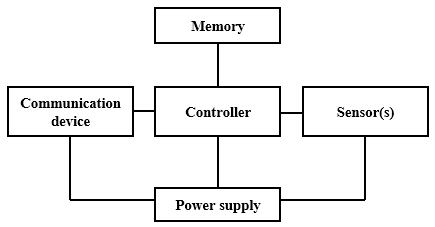
\includegraphics[scale = 1]{images/sensor-node-architecture.png}
		\caption{Sensor Node Architecture}
		\label{fig:sensor-node-architecture}
	\end{figure}

	\begin{description}
	\item[Controller] is the Central Processing Unit (CPU) of the node.
		It collects data from the sensors, processes this data, decides when and where to send it, receives data from other sensor nodes, and decides on the actuator’s behavior.
		It executes various programs, ranging from time-critical signal processing and communication protocols to application programs.
	
	\item[Communication Device] is used to exchange data between individual nodes at radio frequency.
		Radio Frequency (RF)-based communication is widely used in sensor networks as it best fits the requirements of numerous applications.
		It provides relatively long range and high data rates, acceptable error rates at reasonable energy expenditure, and does not require line of sight between sender and receiver.
		Both a transmitter and a receiver are required in a sensor node. 
		The essential task for the devices is to convert a bit stream coming from a microcontroller (or a sequence of bytes or frames) and convert them to and from radio waves. 
		It is convenient to use a device that combines these two tasks in a single entity, called transceivers. 
		Usually, half-duplex operation is realized since transmitting and receiving at the same time on a wireless medium is impractical in most cases.

	\item[Sensors] can be roughly categorized into three categories.
		\textit{Passive, omnidirectional sensors} can measure a physical quantity at the point of the sensor node without actually manipulating the environment by active probing in this sense, they are passive. 
		Moreover, some of these sensors actually are self-powered in the sense that they obtain the energy they need from the environment – energy is only needed to amplify their analog signal. 
		There is no notion of ``direction'' involved in these measurements.
		Typical examples for such sensors include thermometer, light sensors, vibration, microphones, humidity, mechanical stress or tension in materials, chemical sensors sensitive for given substances, smoke detectors, air pressure, and so on.
		\textit{Passive, narrow-beam sensors} are passive as well, but have a well-defined notion of direction of measurement. 
		A typical example is a camera, which can ``take measurements'' in a given direction, but has to be rotated if need be.
		\textit{Active sensors} are the last group of sensors actively probes the environment, for example, a sonar or radar sensor or some types of seismic sensors, which generate shock waves by small explosions.
		These are quite specific – triggering an explosion is certainly not a lightly undertaken action – and require quite special attention.

	\item[Power supply of sensor nodes] is a crucial system component which has two main aspects.
		First, storing energy and providing power in the required form; second, attempting to replenish consumed energy by ``scavenging'' it from some node-external power source over time.
		Storing power is conventionally done using batteries, the normal AA battery stores about 2.2–2.5 Ah at 1.5 V.
		To ensure truly long-lasting nodes and wireless sensor networks, such a limited energy store is unreliable. 
		We can use energy from a node’s environment ``energy scavenging''.
		For example, \textit{Vibrations} is almost pervasive form of mechanical energy: walls or windows in buildings are resonating with cars or trucks passing in the streets, machinery often has low frequency vibrations, ventilations also cause it, and so on.
		The available energy depends on both amplitude and frequency of the vibration.
		\textit{Pressure variations} is similar to vibrations, a variation of pressure can also be used as a power source. 
		Such piezoelectric generators are in fact used already. 
		One well-known example is the inclusion of a piezoelectric generator in the heel of a shoe, to generate power as a human walks about \cite{shenck2001energy}. 
		This device can produce, on average, 330 $\mu W / cm^{2}$. 
		\textit{Photovoltaics} effect is used in the solar cells can be used to power sensor nodes.
		\textit{Temperature gradients} effect utilizing the differences in temperature can be directly converted to electrical energy.

	\item[The memory component] is fairly straightforward. 
		Random Access Memory (RAM) is used to store intermediate sensor readings, packets from other nodes, and so on. 
		While RAM is fast, its main disadvantage is that it loses its content if power supply is interrupted. 
		Program code can be stored in Read-Only Memory (ROM). 
		Correctly dimensioning memory sizes, especially RAM, can be crucial with respect to manufacturing costs and power consumption.
	\end{description}

\section{Energy Consumption}

	The sensor network's lifetime can be maximized by minimizing the power consumption of communication devices (or transreceiver ) of the sensor nodes.
	The transreceiver is responsible for all the wireless communications between nodes.
	To estimate the power consumption, we have to consider the communication and computation power consumption.
	The transreceiver's energy dissipation depends on two main parameters \cite{wang2002energy}.
	The first is $E_{elec} (J/b)$, the energy dissipated to run the transmit or receive electronics.
	The second is $\varepsilon_{amp} (J/m^2 b)$, the energy dissipated by the transmit power amplifier to achieve an acceptable signal to noise ratio $E_{b} / N_{o} $ at the receiver.
	We assume the $d^2$ energy loss for transmission between sensor nodes since the distances between sensors are relatively short \cite{ettus1998system}. 
	To transmit a $k$ - bit packet at distance $d$, the energy dissipated is:
	\begin{equation}
		E_{tx}(k, d) = E_{elec} \cdot k + \varepsilon_{amp} \cdot k \cdot d^{2}
	\end{equation}
	and to receive the k - bit packet, the radio expends
	\begin{equation}
		E_{rx}(k) = E_{elec} \cdot k
	\end{equation}
	For $\mu Amp$\ wireless sensor, $E_{elec} = 50nJ/b$\ and $\varepsilon_{amp} = 100pJ/m^2 b$.

	Transreceiver can be put into different states to save energy \cite{karl2007protocols}.
	It can be in either transmit or receive state and energy consumption of those states are describe above.
	It can be in Idle state where it is ready to receive packet but is not currently receiving anything.
	It can be in Sleep state where majority of the parts are switched off, and is not able to receive immediately. 
 	To sustain the sensor network for longer times all aspects of the sensor network should be efficient.
	For example, the networking algorithm for routing should be such that it minimizes the distance $d$\ between the nodes.
	The signal processing algorithm should be such that it process the networking packets with less computations.
	It is shown in \cite{wang2002energy} that by distributing the Fast Fourier Transform (FFT) algorithm in the network requires less communication between the sensor nodes.
	Also, for minimal energy dissipation, a processor should operate at the lowest voltage for a given clock frequency.

\section{Resource Constraints}
	\label{sec:aggregate-adversary}
	We introduce the parameters which should be taken into account while designing secure protocol for sensor networks.  
	These parameters can constrain the protocol designer's choices within the protocol.

	\subsection{Physical Limitations}
		Sensor nodes are often deployed in open, hostile and unattended environments, so they are vulnerable to physical tampering due to the lower physical security.
		An adversary can obtain the confidential information from a compromised sensor and reprogram it with malicious software.
		The compromised node may then report an arbitrary false sensor readings to its parent node in the tree hierarchy, making the sensor readings unreliable and irrelevant	.
		This attack becomes more damaging when multiple adversaries succeeds in injecting false data into the network which may cause catastrophic consequences \cite{wagner2007algorithms}.	

	\subsection{Hardware Limitations}
		As far as we know, one of the first hardware platform for developing sensor network application is MICA \cite{hill2002mica} developed by University of Berkeley.
		Another popular platform is Mote from Intel \cite{arazi2006self}.
		Due to lower manufacturing cost of sensor nodes, they have low speed processor, limited storage, a short range trans receiver.
		For example, the major specifications for the latest ZigBee chip supporting IEEE 802.15.4 standard, CC2538 from Texas Instruments are shown in Table \ref{table:soc}.
		This chip can do most of the security algorithms but has really little amount of memory storage. It has limited output power which constraints its transmission range which forces us to use multi-hop routing in the network as one node can not communicate with the node outside of its transmission range.
		These hardware limitations can constrain protocol designer's choice of algorithms for applications.  
		\begin{table}[!htb]	
			\begin{center}
				\begin{tabular}{ |l| l| }
					\hline
				     & CC2538 \\
				    \hline
				    Device Type & Wireless Micro controller \\
				    Frequency & 2.4GHz \\
				    Processor Integration & ARM Cortex-M3 \\
						Flash & Up to 512 KB \\
						RAM & Up to 32 KB \\
						Security & AES-128/256;ECC-128/256; SHA2; RSA \\
						RX Current & 20 (mA) \\
						Output Power & 7 (dBm) \\
						Data Rate(Max) & 250 kbps \\
						Type of Battery & AAA; AA; Rechargable(Li-ION) \\
				    \hline
				\end{tabular}
			\end{center}
			 \caption{System-on-Chip specifications for CC2538 from Texas Instruments implementing IEEE 802.15.4 standards}
			 \label{table:soc}
		\end{table}
	
	\subsection{Transmission Medium}
		In sensor networks, a group of sensor nodes ( or processors ) communicate over the radio (e.g., Bluetooth, WLAN).
		Traditionally, wireless mediums have issues due to synchronization, hidden station and expose station terminal problems, distributed arbitration, directional antennas, bandwidth limitations, higher error rate, security, scalability etcetera.
		For example, wireless networks have approximately $10^6$ times higher bit error rate (BER) than wired networks which causes frequent link loss and then path loss. 
		Hence, making unstable routing in the network.
		Higher BER creates higher collision rate in the network, generating higher overhead of retransmission and lowering the channel utilization and the throughput of the network.
		This kind of transmission medium with constrained resources makes it challenging to design the reliable networking protocol as we have to consider all the possible retransmissions.

	\subsection{Mobility}
		As we know, sensor nodes communicate via radio and the availability of the transmission medium changes over time due to link failure, bandwidth limitations or change in network topology.
		Nodes may be able to move, which further contributes to the instability of the communication link.
		The mobility issue makes difficult to do the routing in the network with the directional antennas in place.
		It also requires network to be agile enough to do the reconfiguration for the newer network topology.
		It impedes while doing the quality of service in the network. 
		
	All these parameters combined contributes to making strong assumptions on the network topology while designing the protocol for sensor networks.
\chapter{Networking and Cryptography tools} % (fold)
\label{cha:Networking and Cryptography tools}
	Here we describe the networking and cryptographic tools used in this protocol referred from \cite{menezes2010handbook,stinson2005cryptography}.
	For example, we describe the Hash function, its properties and how it helps us achieve data integrity.

\section{Cryptography}
	The word cryptography means ``secret writing'' and is the art and science of concealing meaning.
	Cryptoanalysis is the breaking of codes.
	The basic component of cryptography is a cryptosystem \cite{bishop2004introduction}.
	\begin{definition}
		A cryptosystem is a $5$-tuple ($ \mathcal{E,D,M,K,C}$), where $\mathcal{M}$ is the set of \textit{plaintexts}, $\mathcal{K}$ is the set of \textit{keys}, $\mathcal{C}$ is the set of \textit{ciphertexts}, $\mathcal{E}:\mathcal{E} \times \mathcal{K} \rightarrow \mathcal{C}$ is the set of \textit{enciphering functions}, and $\mathcal{D}:\mathcal{C} \times \mathcal{K} \rightarrow \mathcal{M}$ is the set of \textit{deciphering functions}.
	\end{definition}

	Classical cryptosystem (also called symmetric cryptosystem or single-key cryptosystem) are cryptosystem that use the same key for encipherment and decipherement.
	In these system, for all $E_{k} \in \mathcal{C}$ and $k \in \mathcal{K}$, there is a $D_{k} \in \mathcal{D}$ such that $D_{k} = E_{k}^{-1}$
\section{Encryption}

\section{Hash Function}
	A hash function takes a message as its input and outputs a fixed length message called hash code.
	The hash code represents a compact image of the message like a digital fingerprint.
	Hash functions are used to achieve data integrity.

	A hash function $h$ should have the following properties:
	\begin{itemize}
		\item Compression - $h$ maps an input $x$ of arbitrary finite bitlength, to an output $h(x)$ of fixed bitlength $n$.
		\item Ease of computation - given $h,x$ it is easy to compute $h(x)$.
		\item Preimage resistance - for all pre-specified outputs, it is computationally infeasible to find any input which hashes to that output, i.e., to find any preimage $x'$ such that $h(x') = y$ when given $y$ for which a corresponding input is not known.
		\item 2nd-preimage resistance - it is computationally infeasible to find any second input which has the same output as any specified input, i.e, given $x$, to find a 2nd-preimage $x' \neq x$ such that $h(x') = h(x)$.
		\item Collision resistance - it is computationally to find any two distinct inputs $x,x'$ which hash to the same output, i.e., such that $h(x) = h(x')$.
	\end{itemize} 

	We use SHA-$256$\cite{SHA256} hash algorithm as a collision resistant hash function.
	% cite NIST for SHA-256

\section{Digital Signatures}
	\label{sec:digital-signature}
	A digital signature is a mathematical scheme for demonstrating the authenticity of a digital message. 
	A valid digital signature gives a recipient reason to believe that the message was created by a known sender, such that the sender cannot deny having sent the message (authentication and non-repudiation) and that the message was not altered in transit (integrity).
	A Digital Signature scheme consists of the following:
	\begin{enumerate}
		\item a plain text message space $\mathcal{M}$ (set of strings over alphabets)
		\item a signature space $\mathcal{S}$ (set of possible signatures)
		\item a signing key space $\mathcal{K}$ (set of possible keys for signature generation) and a verification space $\mathcal{K^{'}}$ (a set of possible verification keys)
		\item an efficient key generation algorithm \textsf{Gen} : $N \rightarrow$ $\mathcal{K} \times \mathcal{K^{'}} $ 
		\item an efficient signing algorithm \textsf{Sign} : $ \mathcal{M} \times \mathcal{K} \rightarrow \mathcal{S}$
		\item an efficient verification algorithm \textsf{Verify} : $\mathcal{S} \times \mathcal{M} \rightarrow$ \{true, false\} 
	\end{enumerate}
	For any secret key $s_{k} \in \mathcal{K}$ and any $m \in \mathcal{M}$,	the message $m$ is signed using key $s_{k}$ as follows:
		\begin{equation}
			s = \textsf{Sign}_{s_{k}}(m)
			\label{eq:signature}
		\end{equation}
	For any $s_{k}$ let $p_{k}$ denote public key and for all $m \in \mathcal{M}$ and $s \in \mathcal{S}$, $s$ as follows:
	\begin{equation}
		\textsf{Verify}_{p_{k}}(m,s) = 
		\begin{cases}
		 \textbf{true}\ \mbox{with probability of 1} & if\ s = \textsf{Sign}_{s_{k}}(m)\\
		 \textbf{false}\ \mbox{with overwhelming probability} & if\ s \neq \textsf{Sign}_{s_{k}}(m)
		\end{cases}
		\label{eq:verification}
	\end{equation}
	where the probability space is determine by the $\mathcal {M, S, K, K^{'}}$ and perhaps the signing and verification algorithms.
	The ``overwhelming probability'' for the signature scheme determines the probability that the scheme allows for a forgery.
	Note that the Digital Signature scheme satisfies the following requirements:
		\begin{itemize}
			\item Only the owner of the secret key can generate a valid signature.
			\item The digital signature is easily verified by other parties.
			\item The digital signature is not only tied to the signer but also to the message that is being signed.
			\item Digital signatures cannot be separated from the message and attached to another message.
			\item Digital signatures do not encrypt the message. However, if necessary, a signed message can be encrypted after it is signed.
		\end{itemize}
	The Figure \ref{fig:digita-signature} from \cite{DigitalSignature}, shows the steps for signing and verifying the hashed message. 
	\begin{figure}[h!]
		\centering
		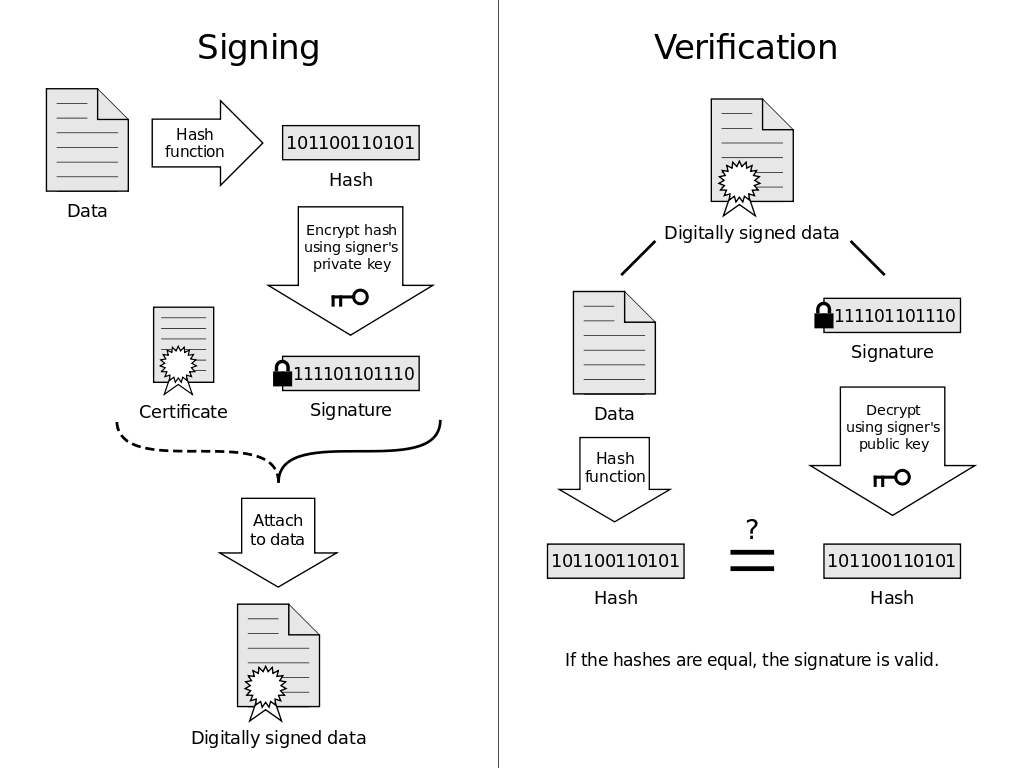
\includegraphics[scale = 0.4]{images/Digital_Signature_diagram.png}
		\caption{ Signing and verification of digital signatures}
		\label{fig:digita-signature}
	\end{figure}
	The message is hashed before its being signed to reduce the message size. 
	If the message is not hashed before signing then the signature can be longer than the message which is problematic for the longer messages.
	\textbf{Talk about non-repudiation, authenticity, integrity.}
	\textbf{Talk about similarities and differences between physical world signature non-repudiation, authenticity, integrity.}
	In physical world, your signatures are the same for all the messages. 
	But this can not be possibly true for digital signatures as the attacker can obtain one signature and then use the same signature to pretend some one else.

\section {Tree generation algorithms}

\section{XOR function}

\section{Elliptic curve}
\chapter{In-network Data-Aggregation Overview} % (fold)
\label{cha:In-network Data-Aggregation Overview}

\section{In network aggregation}
	Sensor networks are being used in scientific data collection, fire alarm systems, traffic monitoring, wildfire tracking, wildlife monitoring and many other applications.
	In sensor networks, thousands of sensor nodes interact with the physical environment and collectively monitors an area, generating a large amount of data to be transmitted and reason about.
	The sensor nodes in the network often have limited resources, such as computation power, memory, storage, communication capacity and most significantly, battery power.
	Also, data communication between nodes consumes a large portion of the total energy consumption. 
	The in-network data aggregation reduces the energy consumption by eliminating redundant data being transmitted to the base station.
	For example, in-network data aggregation of the \textit{SUM} function can be performed as follows. 
	Each intermediate sensor node in the network forwards a single sensor reading containing the sum of all the sensor readings of all of its descendants, rather than forwarding each descendants sensor reading one at a time to the base station.
	It is shown that the energy-savings achieved by in-network data-aggregation are significant \cite{madden2002tag}.
	The in-network data aggregation approach requires the sensor nodes to do more computations.
	But studies show that data transmission requires more energy than data computation. 
	Hence, in-data aggregation is an efficient and widely used approach for saving bandwidth by doing less communications between sensor nodes and ultimately giving longer battery life to sensor nodes in the network.

	We define following terms to help us define goals of in-network data-aggregation approach.
	\begin{definition}\label{def:payload}
		\textbf{Payload} is the part of the transmitted data which is the fundamental purpose of the transmission, to the exclusion of information sent with it such as metadata solely to facilitate the delivery.
	\end{definition}
	\begin{definition}\label{def:information-rate}
		\textbf{Information-rate} for a given node is the ratio of the \payloads, number of \payloads\ sent divided by the number of \payloads\ received.
	\end{definition}
	The goal of the aggregation process is to achieve lowest possible \informationRate.
	In the following section, we show that reducing \informationRate\ makes the intermediate (aggregator) sensor nodes more powerful. Also, it makes aggregated \payload\ more fragile and vulnerable to various security attacks.

\section{Security in In-network data aggregation}
	In-network data aggregation approach saves bandwidth by transmitting less \payloads\  between sensor nodes but it gives more power to the intermediate aggregator sensor nodes. 
	For example, an intermediate malicious sensor node who is doing aggregation over all of its descendants \payloads, needs to tamper with only one aggregated \payload\ instead of tampering with all the \payloads\ from all of its descendants. 
	It means an intermediate malicious sensor node needs to do less work to skew the final aggregated \payload.
	Also, an adversary controlling few sensor nodes in the network can cause the network to return unpredictable results, making an entire sensor network unreliable.
	Notice that, the more descendants an intermediate sensor node has the more powerful it becomes.
	Despite the fact that in-network aggregation makes an intermediate sensor nodes more powerful, many in-network aggregation schemes assumes that all the sensor nodes in the network are honest \cite{yao2002cougar, madden2003design}.

In network aggregation in a single hop network cite papers.

In network aggregation in a  multi hop network cite papers.

Payload, information rate.


\chapter{Aggregate Commit with Verification} % (fold)
\label{cha:A Protocol for Commitment Tree Generation}
\section{Motivation}	
	In the previous chapter, we saw that SHIA limits the adversary's ability to manipulate the aggregation result with the tightest bound possible.
	But, SHIA uses truncated sum as an aggregate function which is resilient according to the Wagner \cite{wagner2004resilient}.
	Furthermore, SHIA does not help detecting and revoking the malicious aggregate node from the network.
	% SHIA does not require prior knowledge of network topology and works on hierarchical sensor network which might include multiple malicious sensor nodes, with only suboptimal congestion overhead.
	% SHIA helps the sensor node verify, its reported sensor reading was aggregated correctly or not, by an an aggregate node.
	% If an an aggregate node has tampered with the reported sensor reading then the relevant sensor node can detect the tampering and raise an alarm.
	We develop the aggregation protocol which works for any random hierarchical sensor networks with a single or multiple adversaries.
	The algorithm works on the resilient as well as non-resilient aggregation functions Defined in \ref{def:resilient}, without compromising any desired security properties.
	Our protocol helps identify the malicious aggregate node or nodes in the network who are responsible for it.
	We want to prevent masquerade attacks in the network to apply this protocol in the voting applications.
	We want to achieve all these desired security properties by inducing only $O(\delta \log^{4} n)$ node congestion in the aggregation tree; where $n$ is the number of nodes in the network, and $\delta$ is the fanout of any node in the aggregation tree.
	use $k$ in the power of log.
	% which is built on top of commitment tree generation of SHIA mentioned in the previous chapter.
	
	The high level idea of the aggregate commit with verification scheme is that all the leaf nodes in the aggregation tree sends the signature of their data-item signed by themselves, in addition to the data-item.
	The aggregate node proceeds to the aggregation only after verifying all the received the data-items.
	The aggregate node also signs its payload in addition to its data-item which is discussed in great detail in the following sections.

\section{Data-Item}
	
	Here, we describe structure of the data-item, how it is different from the label structure of SHIA and rational behind it.	
	\begin{definition}
		\label{def:data-item}
		A commitment tree is a binary tree where each vertex has an associated data-item representing the data that is passed on to its parent. The data-items have the following format:

		$\hspace{100pt}$ \textbf{$<\ $id, count, value, commitment$\ >$}
	\end{definition}
	Where $id$ is the unique ID of the node; $count$ is the number of leaf vertices in the subtree rooted at this vertex; $value$ is the SUM aggregate computed over all the leaves in the subtree and $commitment$ is a cryptographic commitment.
	
	We remove the $complement$ field from the label structure Defined \ref{def:label}. 
	We think including the complement filed in the label is redundant information. 
	The complement field is used by the base station (the querier according to SHIA), before the result checking phase, to verify \textbf{SUM + COMPLEMENT =} $\textbf{n} \cdot \textbf{r}$ ; where $\textbf{n}$ is the number of nodes in the network, $\textbf{r}$ is the upper bound on the allowed sensor readings.
	We can achieve the same upper bound without the complement field.
	As the querier knows $n, r$ and it gets SUM from the root of the aggregation tree.\\
	If \textbf{SUM} $> \textbf{n} \cdot \textbf{r}$ , then the base station knows some node or nodes in the network reported out of range readings.

	We include $id$ of the node in its data-item.
	SHIA does not have the ID field in their label structure as they do not do internal verification while creating a commitment tree.
	In the label format ID of the node is hashed after the first aggregation and virtually gets lost.
	We do internal verification so it is necessary for any aggregate node to know the ID of all the received data-items in its forest, for the verification of the received signatures.

\section{Signing the Data-Item}
	There is one vertex $S_{0}$ for each sensor node $S$, which we call the leaf vertex of $S$.
	The data-item for leaf vertex $S_{0}$ is defined according to Equation \ref{eq:leaf-vertex} and associated signature to it is defined according to Equation \ref{eq:signature-leaf-vertex}.
	\begin{equation}
		\label{eq:leaf-vertex}
		S_{0}\ =\ <S_{id}, 1, S_{value}, H(N||1||S_{value})>
	\end{equation}
	\begin{equation}
		\label{eq:signature-leaf-vertex}
		\textsf{Sign}_{S_{S}}(S_{0})
	\end{equation}
	where $H$ is a collision resistant hash function, $S_{S}$ is the secret key of $S$, $N$ is the query nonce.
	In aggregate commit with verification scheme, in addition to sending the data-item, each sensor node sends the signature of the data-item to its parent.
	The parent node verifies all the received signature and then proceeds to the aggregation.
	
	\subsection{Security Benefits}
		\begin{itemize}
			\item A sensor node has the proof for the sent data-item and can not claim sending the different data-item to its parent in the future.
			\item Each data-item has an associated signature to it, which helps an aggregate node verify the authenticity of the data-item.
			\item The parent node has the proof for the received data-item, and can not claim receiving different data-items form its children in the future.
		\end{itemize}

\section{Signing the Commitment Payload}
		We define commitment payload based on the commitment forest Defined in \ref{def:commitment-forest}.
	\begin{definition}
		A \textbf{commitment payload} is a set of data-items of the root vertices of the trees in the outgoing commitment forest.
	\end{definition}
	% We use the term payload for commitment payload and the term forest for the commitment forest.
	For brevity, we use the term forest, payload instead of commitment forest, commitment payload respectively.
	In addition to sending all the data-items with their respective signatures, an aggregate node sends an additional signature to its parent, which is a signature of all the data-items in its payload.
	% Each sensor node signs all the data-items in its commitment payload before sending it to its parent.
	% to prove the fact that it has verified all the data-items in its commitment forests.
	\begin{exmp}
	The aggregation tree shown in Figure \ref{fig:Palm aggregation tree}, the payload of sensor node $C$ is show in Figure \ref{fig:commitment-tree-example-1}.
			\begin{figure}[h!]
				\centering
				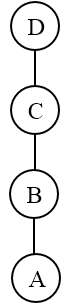
\includegraphics[scale = 0.5]{images/palm-aggregation-tree.png}\\
				\caption{Palm aggregation tree}
				\label{fig:Palm aggregation tree}
			\end{figure}
		% $C$ receives $B_{1}$, $Sign(B_{1})$ from $B$.
		% And $C$'s commitment forest is show in Figure \ref{fig:Commitment forest of C}.
		% $B_{1} = <B_{id}, 2, B_{value}, H(N||2||B_{value}||A_{0}||B_{0})>$; $Sign(B_{1}) = E_{K_{B}}(H(B_{1}))$\\
		% 	\begin{figure}[h!]
		% 		\centering
		% 		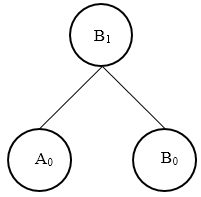
\includegraphics[scale = 0.5]{images/commitment-forest-of-C.png}\\
		% 		\caption{$C$'s commitment forest }
		% 		\label{fig:Commitment forest of C}
		% 	\end{figure}\\
		The sensor node $C$ sends all the data-items in its payload with their signatures to its parent sensor node $D$.
		Furthermore, $C$ sends the signature of its payload $\textsf{Sign}_{S_{C}}(C_{0}||B_{1})$ to $D$.\\
			\begin{figure}[h!]
				\centering
				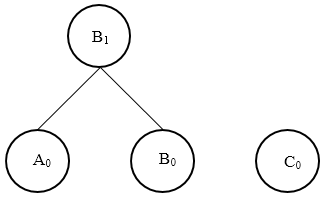
\includegraphics[scale = 0.5]{images/commitment-payload-of-C.png}
				\caption{$C$'s commitment commitment-payload}
				\label{fig:Commitment payload of C}
			\end{figure}
		\begin{equation}	
			\begin{array}{l}
				B_{1} =\ <B_{id}, 2, B_{1value}, H(N||2||B_{1value}||A_{0}||B_{0})>; \textsf{Sign}_{S_{B}}(B_{1})\\
				C_{0} =\ <C_{id}, 1, C_{value}, H(N||1||C_{value})>; \textsf{Sign}_{S_{C}}(C_{0})\\
				\textcolor{red}{\textsf{Sign}_{S_{C}}(C_{0}||B_{1})}
			\end{array}
		\end{equation}
	% Sending an additional signature with all the data-items signifies that a sensor node has verified all the data-items.
	% The basic idea is that the sensor node signs all the data-items it sends to its parent.
	% \textbf{Because of the signature, the sensor node has the proof for the sent data-item.
	% It also prevents the parent or ancestor node from claiming the different received data-item.}
	\end{exmp}
	\subsection{Security Benefits}

	This additional signature signifies the following:
	\begin{itemize}
		\item	An intermediate sensor node has verified all the data-items in its forest before creating its payload.
		\item From the parent node perspective, it has received all the verified data-items from the signer node and not from anywhere else.
		% \item From the parent or ancestor node perspective, it has received all the verified data-items from its children and not from anywhere else.
	\end{itemize}

	\section{Commitment Tree Generation}
	For the given aggregation tree the commitment forest is built as follows.
	Leaf sensor nodes in the aggregation tree create their leaf vertex by creating data-items and their respective signatures according to Equation \ref{eq:leaf-vertex}, \ref{eq:signature-leaf-vertex} which they send it to their parent as a payload in the aggregation tree.
	Each internal sensor node $I$\ in the aggregation tree also creates their leaf vertex and its signature.
	In addition, $I$\ receives the payload from each of its children which creates the forest for $I$.
	Once $I$ verifies all the received signatures, it merges all the data-items in its forest with same count value to create its payload.
	Note that we can determine the height of the commitment tree from the count value.

	Suppose $I$ have to create its payload by merging $i$ data-items $D_{1}$, $D_{2}$, $\dotsc$, $D_{i}$ in its forest.
	First, $I$ verifies the received signatures $Sign(D_{1})$, $Sign(D_{2})$, $\dotsc$, $Sign(D_{i})$.
	Once verified, $I$ starts merging the data-items as follows.
	Let $c$ be the smallest count value in $I$'s forest.
	The sensor node $I$ finds two data-items $D_{1},D_{2}$ in its forest with the same count value $c$ and merges them into a new data-item with the count of $c+1$ as shown in Figure \ref{fig:increase-height}.
	\begin{figure}[h!]
		% \centering
		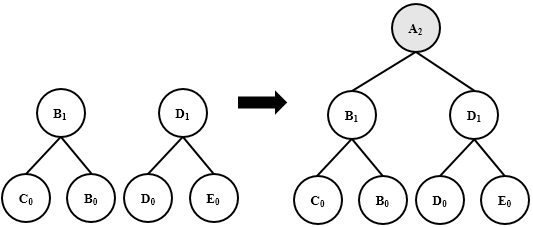
\includegraphics[scale = 1]{images/increase-height.png}\\
		\caption{$A$ has $B_{1}, C_{1}$ in his forest and aggregates those two trees and creates $A_{2}$.}
		\label{fig:increase-height}
	\end{figure}\\
	It repeats the process until no two data-items in its forest have the same count value.
	An example of generating the payload by merging the data-items in the forest for the sensor node $A$ in Figure \ref{fig:at} is illustrated in the following example.
	% \ref{fig:commitment-tree-example-1}, \ref{fig:commitment-tree-example-2}, \ref{fig:commitment-tree-example-3}, \ref{fig:commitment-tree-example-4}.
			\begin{exmp} The commitment-payload generation process for node $A$ of Figure \ref{fig:at} is shown here.\\
				\begin{figure}[h!]
					\centering
					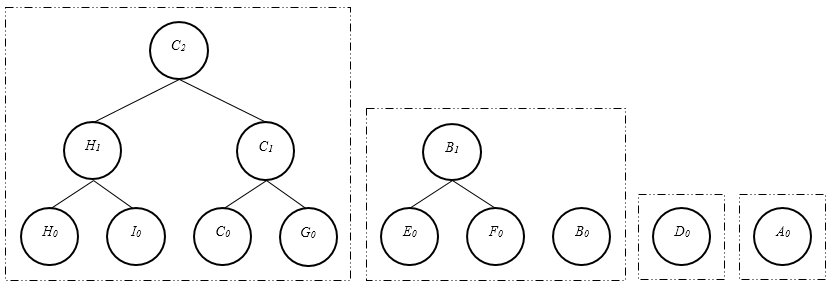
\includegraphics[scale = 1]{images/commitment-tree-example-1.png}\\
					\caption{$A$ receives $C_{2}$ from $C$, $(B_{1},B_{0})$ from $B$, $D_{0}$ from $D$ and generates $A_{0}$. The commitment payload received from a given sensor node is indicated by dashed-line box.}
					\label{fig:commitment-tree-example-1}
				\end{figure}
				\begin{equation}
					\begin{array}{l}
						A_{0} = <A_{id}, 1, A_{value}, H(N||1||A_{value})>; \textsf{Sign}_{S_{A}}(A_{0}) \\
						D_{0} = <D_{id}, 1, D_{value}, H(N||1||D_{value})>; \textsf{Sign}_{S_{D}}(D_{0})\\
						B_{0} = <B_{id}, 1, B_{value}, H(N||1||B_{value})>; \textsf{Sign}_{S_{B}}(B_{0})\\
						B_{1} = <B_{id}, 2, B_{value}, H(N||2||B_{value}||E_{0}||F_{0})>; \textsf{Sign}_{S_{B}}(B_{1})\\
						\textcolor{red}{\textsf{Sign}_{S_{B}}(B_{0} || B_{1}), benefits}\\
						C_{2} = <C_{id}, 4, C_{value}, H(N||4||C_{value})||H_{1}||C_{1})>; \textsf{Sign}_{S_{C}}(C_{2})\\
						\end{array}
				\end{equation}

				\begin{figure}[h!]
					\centering
					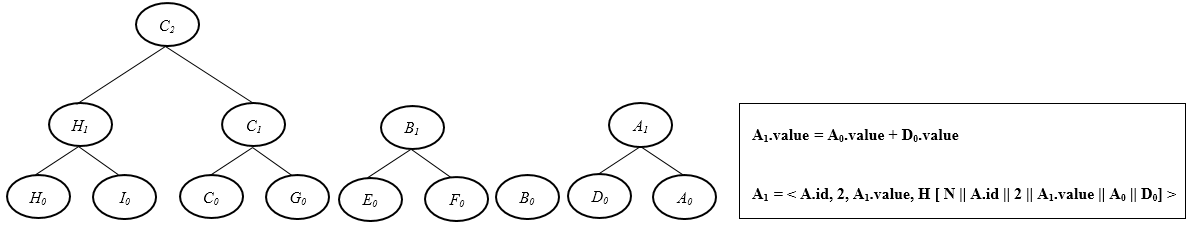
\includegraphics[scale = 1]{images/commitment-tree-example-2.png}\\
					\caption{First Merge: $A_{1}$ vertex created by A.}
					\label{fig:commitment-tree-example-2}
				\end{figure}

				\begin{equation}
					\begin{array}{l}
				A_{1} = <A_{id}, 2, A_{1value}, H(N||2||A_{1value}||A_{0}||D_{0})>; \textsf{Sign}_{S_{A}}(A_{1})\\
				where\  A_{1value} = A_{value} + D_{value} \\
					\end{array}	
				\end{equation}
				\begin{figure}[h!]
					\centering
					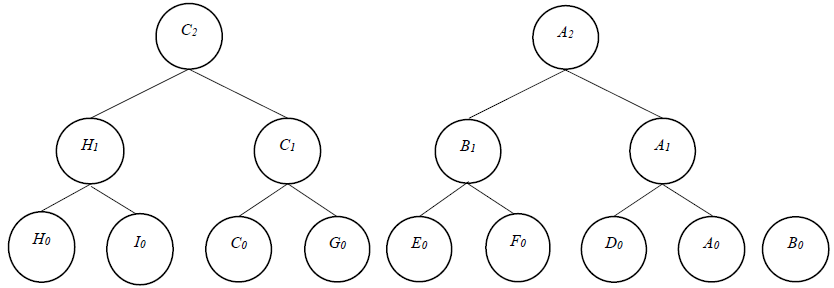
\includegraphics[scale = 1]{images/commitment-tree-example-3.png}\\
					\caption{Second Merge: $A_{2}$ vertex created by A.}
					\label{fig:commitment-tree-example-3}
				\end{figure}
				\begin{equation}
					\begin{array}{l}
						A_{2} = <A_{id}, 4, A_{2value}, H(N||4||A_{2value}||B_{1}||A_{1}) >; \textsf{Sign}_{S_{A}}(A_{2})\\
						where\  A_{2value} = B_{1value} + A_{1value} \\
					\end{array}
				\end{equation}
				\begin{figure}[h!]
					\centering
					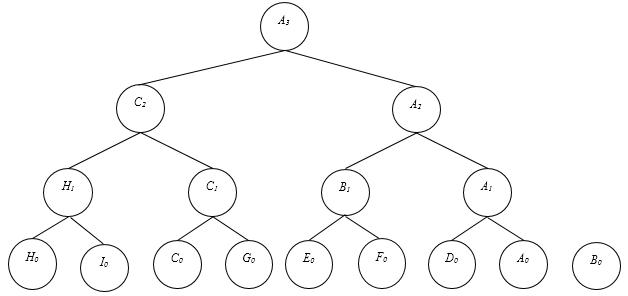
\includegraphics[scale = 1]{images/commitment-tree-example-4.png}\\
					\caption{Third Merge: $A_{3}$ vertex created by A.}
					\label{fig:commitment-tree-example-4}
				\end{figure}
				\begin{equation}
					\begin{array}{l}
						A_{3} = <A_{id},8, A_{3value},H(N||8||A_{3value}||C_{2}||A_{2})>; \textsf{Sign}_{S_{A}}(A_{3})\\
						where\ A_{3value} = A_{2value} + C_{2value}
					\end{array}
				\end{equation}
			\end{exmp}
% chapter A Protocol for Commitment Tree Generation (end)

% Talk about the certificates:
	
% 	How many certificates does $A$ need to know in this example ?
% 	In the above example, $A$ need to know $D,B,C's$ certificate to verify their signatures.
% 	But if we use SHIA'a approach of creating commitment tree then $A$ need to know $E's$ certificate as well.
% 	Hence, being root in as many tree as possible is the more efficient.
\section{Bandwidth Analysis}
	For any given sensor node's forest with $n$ leaf vertices, has at most $\log n$ data-items in its payload.
	It has at most $(\log n) +1$ signatures in its payload.
	The highest possible count value is $\log n$, as all the trees are binary. 

	An intermediate sensor node $S$ with $\beta$ descendants in the aggregation tree, has at most $\log(\beta+1)$ data-items with their respective $\log(\beta+1)$ signatures in its payload.
	$S$ might need to send its payload signature $Sign(S_{p})$.
	At max, $S$ has to send a payload with $\log(\beta+1)$ data-items and $\log(\beta+1) +1$ signatures to its parent in the aggregation tree.
	
	Hence, sending signatures of the data-items causes $O(\log \beta)$ bandwidth overhead for each node in the network, where $\beta$ is the number of descendants of the sensor node. 

\section{Performance Analysis}
	In addition to calculating its own data-items, all intermediate sensor nodes with $\beta$ descendants and $\zeta$ direct children need to do the following:
	\begin{itemize}
		\item To calculate and verify $O(\log \beta)$ signatures, creating $O(\log \beta)$ calculation overhead. 
		\item Needs sufficient memory to cache $O(\log \beta)$ certificates. 
		\item Needs enough memory to cache $\Omega(\zeta)$ certificates.
	\end{itemize}

	% Computation cost: Needs to calculate that many signatures. Needs to verify that many signatures.
	% Need to know that many certificates.

\section{Applications}
		The signature based aggregation scheme can be applied to do the \textbf{voting} in the network.
		And voting scheme can be used to solve many sensor network problems.
		For example, voting can be used to design the distributed algorithm for selecting a cluster head or node revocation system.
		In the voting scheme, following are the major security concerns: 
		\begin{itemize}
			\item The aggregate node needs to know that the vote is coming from the legit voter, no other voter is impersonating the vote of the legit voter.
			\item Only the intended aggregate node should be able to verify the vote.
			\item The aggregate node should not be able to tamper with the votes. 
			\item The aggregate node needs the proof that it aggregated the verified votes.
			\item The voter need the proof for which vote it sent to its aggregator.
		\end{itemize}
		For example, the base station wants to know the overall vote-count in the network.
		To do so, all the leaf nodes send their votes and the signature of their votes to their respective aggregate nodes in the network.
		The aggregate nodes receive votes with their signatures from all of their children voters.
		The aggregate nodes verify all the votes and count those votes.
		Then they forward the count and the signature of that count signed by the aggregate node to their respective parent in the aggregation tree.
		This process is repeated until the final count and its signature, is sent to the base station by the root of the aggregation tree.
				
	\textbf{Node power level},
	\textbf{Surveillance Application}

\chapter{SYSTEM DESIGN} % (folit
\label{cha:System Design}
	
	This chapter describes the rationale behind the design specifications of our secure aggregation protocol for sensor networks, the mechanism used to achieve it and implementation details.

	\section{Introduction}

	The most significant design aspect of the sensor network is the \textit{Lifetime of the Network}.
	A sensor network tends to have limited life span as they are powered by the battery.
	The lifetime of the sensor network is inversely proportional to the sensor nodes' power consumption.
	One of the most dominating factor for the power consumption is transmitting and receiving data between sensor nodes, making network bandwidth an expensive resource.
	The bandwidth is a more expensive resource than the local data computation, as trans-receiving activity consumes more power than computation.
	The obvious solution to increase the lifespan of the sensor network is to decrease the bandwidth usage in the network.
	As we know, data aggregation techniques can greatly reduce the bandwidth usage in the network, increasing the lifespan of the network.
	Hence, data-aggregation techniques are one of the key tool in our tool box while designing protocol for the sensor networks.

	The second most significant factor in the design of the data aggregation protocol is \textit{Security Architecture }.
	The International Telecommunications Union (ITU) Telecommunication Standardization Sector (ITU-T) Recommendation X.800, \textit{Security Architect for Open Systems Interconnection} (OSI) provides a systematic approach for it.
	The OSI security architecture focuses on security attacks, mechanism and services defined as follows:
	\begin{description}
		\item[Security attack] is any action that compromises the security of information owned by an organization or entity \cite{stallings2008computer}.
		\item[Security mechanism] is a mechanism that is designed to detect, prevent, or recover from a security attack
		\cite{stallings2008computer}.
		\item[Security service] is a service that enhances the security of the data processing systems and the information transfers of an organization. The services are intended to counter security attacks, by using one or more security mechanisms \cite{stallings2008computer}.

	\end{description}

	Security attacks can be classified as \textit{active attacks} and \textit{passive attacks}.
	
	Active attacks involve some modification of the data stream or the creating of a false stream and can be subdivided into four categories: \textit{replay, masquerade, modification of messages, and denial of service}.
	Replay involves the passive capture of a data unit and its subsequent retransmission to produce an unauthorized effect.
	A masquerade takes place when one entity pretends to be a different entity.
	For example, authentication sequence can be captured and replayed after a valid authentication sequence has taken place, thus enabling an authorized entity with few privileges to obtain extra privileges by impersonating an entity that has those privileges.
	Modification of message means that some portion of a legitimate message is altered or that the messages are delayed or reordered, to produce an unauthorized effect.
	For example, a message stating ``Allow Barack Obama to read confidential file accounts.'' is modified to say ``Allow Michelle Obama to read confidential file accounts.''
	The denial of service inhibits the normal use of communication facilities.
	For example, an entity may suppress all messages directed to a particular destination.
	Another form of service denial is the disruption of an entire network, either by disabling the network or by overloading it with messages so as to degrade performances.
	Active attacks present the opposite characteristics of passive attacks.
	Whereas passive attacks are difficult to detect, measures are available to prevent their success.
	On the other hand, it is quite difficult to prevent active attacks absolutely, because to do so would require physical protection of all communication facilities and paths at all times.
	Instead, the goal is to detect them and to recover from any disruption or delays caused by them.
	Because the detection has a deterrent effect, it may also contribute to prevention.
	
	Passive attacks attempts to learn or make use of information from the system but does not affect the system resources.
	They are in the nature of eavesdropping on, or monitoring of, transmissions.
	% Two types of passive attacks are \textit{release of message contents} and \textit{traffic analysis}.
	% The \textit{release of message contents} is well understood. 
	% A telephone conversation, an electronic mail, and a transferred file may contain sensitive or confidential information.
	% We would like to prevent an opponent from learning the contents of these transmissions.
	% The \textit{traffic analysis} is subtler. 
	% Suppose that we had a way of masking the message so that even if the  opponents captured the message, could not extract it.
	% The common mechanism for masking the message is encryption.
	% If we had encryption protection in place, an opponent might still be able to observe the pattern of these message communication.
	% The opponent could determine the location and identity of communicating hosts and could observe the frequency and length of message being exchanged.
	% These patterns might be useful in guessing the nature of the communication that was taking place.
	Passive attacks are difficult to detect as they do not involve any alteration of the message.
	Typically, the message traffic is sent and received in an apparently normal way and neither the sender nor receiver is aware that a third party has sniffed the message or observed the traffic pattern.
	However, it is feasible to prevent the success of these attacks, usually by means of encryption. 
	Thus, the emphasis on dealing with passive attacks is on prevention rather that detection.
	Passive attacks are subtler and outside the scope of our thesis.

	Security services are divided into six categories:
	\textit{Authentication, Access Control, Data Confidentiality, Data Integrity, Non-repudiation, Availability}.
	
	Authentication service assures that a communication is authenticate.
	Two types of authentication services are described in the standard: \textit{peer entity authentication} and \textit{data origin authentication}.
	The peer entity authentication provides for the corroboration of the identity of a peer entity in an association.
	Two entities are considered as peer if they implement the same protocol in different systems (e.g., two TCP users in two communicating systems).
	Peer entity authentication is used at the establishment of, or at times during the data transfer phase of, a connection.
	It attempts to provide confidence that an entity is not performing either a masquerade or an unauthorized replay of a previous connection.
	Data origin authentication provides the corroboration of the source of a data unit. 
	It does not provide protection against the duplication or modification of data units.
	This type of service supports applications like electronic mail where there are no prior interactions between the communicating entities.
	
	Data Confidentiality ensures the protection of transmitted data from passive attacks.
	It is also known as secrecy or privacy.
	For example, student grade information is an asset whose confidentiality is considered to be highly important by students.
	In the United States, the release of such information is regulated by the Family Educational Rights and Privacy Act (FERPA).
	Grade information should only be available to students, their parents, and employees that require the information to do their job.
	The other aspect of confidentiality is the protection of traffic flow from analysis.
	This requires that an attacker not be able to observe the source and destination, frequency, length, or other characteristics of the traffic on a communications facility.
	Ensuring confidentiality can be difficult.
	For example, who determines which parties are authorized to access the information?
	By ``accessing'' information, do we mean that an authorized party can access a single bit? the whole collection? pieces of information out of context?
	Can someone who is authorized disclose that information to other parties?\cite{pfleeger2002security}
	
	Data Integrity assures that the only authorized entities can modify the information; where modification means writing, creating, deleting and changing the information.
	A hospital patient's allergy information stored in a database illustrates the several aspects of the data integrity.
	The doctor should be able to trust that the information is correct and current.
	Now, suppose a nurse who is authorized to view and update the information deliberately falsifies the data to cause harm to the hospital.
	The database needs to be restored to a trusted basis quickly, and it should be possible to trace the error back to the person responsible.
	Patient allergy information is an example of an asset with a high requirement for integrity. 
	Inaccurate information could result in serious harm or death to a patient and expose the hospital to massive liability.
	Because the integrity service relates to active attacks, we are concerned with detection rather than prevention.
	If a violation of integrity is detected, then the service may simply report this violation, and some other portion of software or human intervention is required to recover from the violation.
	Alternatively, there are mechanisms available to recover from the loss of integrity of data, as we will review subsequently. The incorporation of automated recovery mechanisms is, in general, the more attractive alternative.
	
	Availability  means that the information of a system being accessible and usable by an authorized parties according to performance specification at appropriate times.
	In other words, if some person or system has legitimate access to a particular set of objects, that access should not be prevented.
	Availability applies to the information and services.
	For example, information or service is available can mean the following. 
	It is present in the usable form, having the enough capacity to meet the service need.
	If it is in wait mode, it is making enough progress, and it has a bounded waiting time, meaning there is timely response to our requests.
	Resources are allocated fairly so that some requests are not favored over the others.
	The service can be used easily and in its intended way.
	Availability addresses the concern raised by the denial of service attacks.
	It depends on proper management and control of system resources and thus depends on access control service and other security services.
	
	Non repudiation service requires neither the sender nor the receiver can deny the transmission.
	Thus, when a message is sent, the receiver can prove that the alleged sender in fact sent the message.
	Similarly, when a message is received, the sender can prove that the alleged receiver in fact received the message.
	This is very important in electronic commerce applications, where it is important that a consumer cannot deny the authorization of a purchase.
	
	Access Control is the ability to restrict and control the access to host systems and applications via communications links.
	To achieve this, each entity trying to gain access must first be identified, or authenticated, so that access rights can be tailored to the individual.
	Login credentials and locks are two analogues mechanism of access control.

	Security mechanisms follow one of the most fundamental principle of Open Design \cite{bishop2004introduction} defined as follows:
	\begin{definition}
		The principle of open design states that the security of a mechanism should not depend on the secrecy of its design or implementation.
		\label{def:open-design}
	\end{definition}
	Designers and implementers of a program must not depend on secrecy of the details of their design and implementation to ensure security.
	Others can ferret out such details either through technical means, such as disassembly and analysis, or through nontechnical means, such as searching through garbage receptacles for source code listings (called ``dumpster-diving'').
	If the strength of the program's security depends on the ignorance of the user, a knowledgeable user can defeat that security mechanism.
	The term ``security through obscurity'' captures this concept exactly.
	This is true of cryptographic software and systems.
	Because cryptography is a highly mathematical subject, and companies who sell these softwares want to keep their algorithms secret. 
	Issues of proprietary software and trade secrets complicate the application of this principle.
	In some cases, companies may not want their designs made public, lest their competitors use them.
	The principle then requires that the design and implementation be available to people barred from disclosing tit outside the company.
	Note that keeping cryptographic keys and passwords does not violate this principle, because a key is not an algorithm.
	However, keeping the enciphering and deciphering algorithms secret would violate it.
	The following security mechanisms may be incorporated into the appropriate protocol layer in order to provide some of the OSI services.
	\textit{Encryption} is the use of mathematical algorithms to transform data into a form that is not readily intelligible.
	The transformation and subsequent recovery of the data depend on an algorithm and zero or more encryption.
	\textit{Digital Signature} appends the data to a cryptographic transformation of data unit that allows a recipient of the data unit to prove the source and integrity of the data unit and protects against the forgery (e.g., by the recipient).
	\textit{Hash functions} provides one way functions to achieve irreversible encryption.
	\textit{Traffic Padding}, \textit{Routing Control}, \textit{Notarization}, \textit{Authentication Exchange} are possible mechanisms as well but they are outside the scope of our thesis.

	% \textit{Traffic Padding} is the insertion of bits into gaps in a data stream to frustrate traffic analysis attempts.

	% \textit{Routing Control} enables selection of particular physically secure routes for certain data and allows routing changes, especially when a breach of security is suspected.

	% \textit{Notarization} is the use of a trusted third party to assure certain properties of a data exchange.

	% \textit{Authentication Exchange} is a mechanism intended to ensure the identity of an entity by means of information exchange.

	As you can see, expectations from secure networking protocol are far-reaching.
	It is very ambitious for any system to have all the above mentioned security services at the same time.
	If we have to achieve all the security services for sensor networks we can make each sensor node signs its reading data and then send data with its signature to its parent.
	The network forwards all the data with their respective signatures to the base station.
	The base station verifies all the signatures and then calculates the aggregate function.
	Clearly, this approach is not practical as it requires $n$ signatures to traverse through the link between the base station and the root node of the network; where $n$ is the number of nodes in the network.
	Which makes that link the bottleneck link of the network. 
	And if that link breaks we loose the entire network connectivity.

	In reality all the security services are not always required.
	For example, \textbf{Protecting banner advertisements on web pages}. 
	The provider of the advertisements do not care if they copy the advertisements and show it to other people.
	So, there is no confidentiality at all.
	But they want to prevent people from changing the advertisements to the different types of advertisements.
	Also, when a client downloads a file from the file server using Internet, he can verify the integrity of the file using the checksum.
	But it is okay if somebody on the network sniffed the downloading activity as far as it did not change the content of the file.
	In this application, a client requires the integrity of the file but the privacy of the client, the file server and the Internet service provider are not required.
	To give an analogy with a physical world application, when a person writes a postcard, he puts his own signature on the it. 
	When that postcard delivers successfully by the postal service, the receiving party can verify the integrity of the message from the handwriting and the signature of the person.
	The postal service knows the sender and the receiver of the postcard.
	It can even read the postcard.
	Again, the integrity is important not the confidentiality.
	In most engineering discipline, it is useful to clarify the requirements carefully before embarking on a project \cite{2002-Stajano-ubiquitous}.
	An important aspect to the computer security, as discussed by Anderson \cite{anderson1993cryptosystems}, that is often ignored: designed the security before careful thought of the needs.
 	It is crucial to find out which security services are desired for the particular application, so we can use the relevant security mechanisms to provide those services.
	
	% In practice, protocol designer finds out the most important security services for the applications before designing the protocol.

	For example, Wagner's work \cite{wagner2004resilient} describes the attacks on standard schemes for data aggregation and introduces the problem of securing aggregation in the presence of malicious or spoofed data.
	He proposes a mathematical theory of security for aggregation.
	The theory quantifies, in a principled way, the robustness of an aggregation operator against malicious data.
	It draws novel connections to statistical estimation theory and to the field of robust statistics.
	He identifies techniques for aggregation that provide robustness against attack. 
	It provides helpful guidance to sensor network implementors or designers in selecting appropriate aggregate functions.

	Secure Information Aggregation (SIA) \cite{przydatek2003sia}  addresses the problem of how to enable secure information aggregation, such that the user accepts the data with high probability if the aggregated result is within a desired bound, but that the user detects cheating with high probability and rejects the result if it is outside of the bound.
	SIA provides statistical security under the assumption of a single-aggregator model.
	In the single-aggregator model, sensor nodes send their data to a single
	aggregator node, which computes the aggregate and sends it to the
	base station.
	This form of aggregation reduces communications only on the link between the aggregator and the base station, and is not scalable to large multihop sensor deployments.
	SIA provides the probabilistic data-integrity service under strong network assumptions.

	Secure Hierarchical In-network Aggregation (SHIA) \cite{chan2006secure}, in many ways enhances Secure Information Aggregation (SIA).
	SHIA presents the provably secure sensor network data aggregation protocol for general networks and multiple adversarial nodes, in compare to SIA which provides probabilistic security for a single aggregate network topology.
	SHIA limits the adversary’s ability to manipulate the aggregation result with the tightest bound possible, with no knowledge of the distribution of sensor data values.
	SHIA provides data-integrity service for any hierarchical sensor networks because of that it can detect malicious activity in the network.

	The third most significant aspect is \textit{Data Integrity}.
	% The data collected from the sensors gets aggregated on the way to the base station.
	% The base station takes an important decision based on the received value.
	Suppose, the sensor network is deployed to measure the certain harmful chemical levels in the lab atmosphere and raise an alarm if the it increases above certain level.
	If the base station fails to raise an alarm because of the false aggregated data, can create catastrophic and lethal situation.
	Hence, the data integrity is so important.
	
	Data integrity can be achieved with the error detection and error correction techniques.
	The first step towards achieving the data integrity in the sensor network is to \textit{detect any malicious activity} in the network.
	The second step is the ability to \textit{locate the malicious node or an adversary} in the network.
	We think detecting a malicious activity without tracing down the malicious node responsible for it, is of no value.
	To give an analogy with the physical world, it is like you know there is a crime in the city and you do not do anything about it.
	Locating the criminals responsible for the crime is mandatory to abolish the crime in the city.
	In similar way, locating the malicious node and removing it from the network is an important security service. 
	Failing to provide such a security service, allows an adversary to continue doing the malicious activity in the future, which makes aggregated sensor data garbage. 
	The network has to redo the all the work to create a response for the query from the base station, which consumes lots of bandwidth. 
	An adversary can repeat this process until the network dies due to low battery power, creating a denial of service attack in the network.
	Hence, detecting a malicious node who is responsible for the malicious activity is equally important.
	If we can track down the malicious node in the network then we can remove that node from the network for all future queries.
	And make sure that all the future queries are not manipulated by any malicious node in the network.
	Hence, the fourth and fifth most significant design aspects of secure aggregation protocol are \textit{detect the malicious activity} (in terms of data aggregation) and can \textit{detect the adversary} in the network, respectively.

	To detect an adversary (or prove someone guilty), we need proof that the adversary is responsible for the malicious activity.	 
	% To achieve our goal, we think the Digital signature is the perfect cryptographic tool.
	Consider the following example showing the analogy with the signature scheme in the physical world, used by the postal services.
	When a postman delivers the package, the receiving party has to sign the document informing that he verified and received the package.
	Since only the receiving party can create his signature, in the future he can not claim of not receiving the package or receiving the damaged or incorrect package. 
	If he claims such, the postal company has the signed document as the proof mentioning that the package was received successfully, by the receiving party.
	The signed document also ensures to the postal company that the postman did not misplace or steal the package.
	The signature scheme used by the postal service promises non repudiation security service.
	% authenticity (assures the origin of the message) and 
	Hence, we require \textit{non-repudiation} security service in the sensor network.

	% With Digital signatures one can achieve \textbf{non-deniability  (non repudiation), authentication, integrity} (assures that only the authorized parties can modify the message) as described in Section \ref{sec:digital-signature}.

\section{System Design Specifications}
	We want to design a secure aggregation protocol which maximizes the \textit{network lifetime}.
	The protocol can be applied to \textit{any hierarchical sensor network}.
	Further, we want protocol to work on \textit{resilient} and \textit{non-resilient} aggregate functions without compromising any desired security properties.
	In addition, We want protocol to be secure with \textit{a single} or \textit{multiple adversaries} in the network.
	Moreover, we want the protocol to protect against any \textit{active attacks}. 
	If the aggregation result is accepted by the base station it should have very high confidence in the result, meaning that we want the highest level of \textit{data integrity} security service in the protocol.
	We need the capabilities to \textit{detect any malicious activity}.
	If there is any malicious activity in the network, we should be able to \textit{locate an adversary} responsible for it, in the network.
	Also, we want the \textit{non-repudiation} security service so neither sender nor receiver can deny the transmission or receiving of the message, which is mandatory to locate an adversary.
	Finally, we want to achieve this with the least amount of \textit{bandwidth and computation} overhead in the network.
	So, the protocol can be easily implemented in the real world sensor networks.
	It is not that difficult to provide mentioned security properties to protect against active attacks in the sensor network. 
	We will show that it requires sub-linear edge congestion to provide these services. 

	% THink about PKI as design and RSA and el-gamal are solutions to it.
	% As we saw in the previous chapter SHIA can detect the malicious activity in the network with only sub-linear edge congestion.
	% So, we built our work on top of SHIA which can detect an adversary.


	% For that we want non-repudiation

	% If there is any malicious activity detect it

	% Locate an adversary	
	% fig:Commitment payload of C to detect an adversary in the network with least amount of overhead in terms of BW and computation.
	% We wanted to achieve that with as realistic as possible. 


% \section{Design Goals}


% 	% In the previous chapter, we saw that SHIA limits the adversary's ability to manipulate the aggregation result with the tightest bound possible.
% 	% But, SHIA uses truncated sum as an aggregate function which is resilient according to the Wagner \cite{wagner2004resilient}.
% 	% It does not help accurately calculating the sum aggregate. 
% 	% Furthermore, SHIA does not help detecting and revoking the from the of Sensor Node malicious aggregate no network.
% 	% SHIA does not require prior knowledge of network topology and works on hierarchical sensor network which might include multiple malicious sensor nodes, with only suboptimal congestion overhead.
% 	% SHIA helps the sensor node verify, its reported sensor reading was aggregated correctly or not, by an an aggregate node.
% 	% If an an aggregate node has tampered with the reported sensor reading then the relevant sensor node can detect the tampering and raise an alarm.
% 	We develop the aggregation protocol which works for any random hierarchical sensor networks with a single or multiple adversaries.
% 	It works on the resilient as well as non-resilient aggregation functions Defined in \ref{def:resilient}, without compromising any desired security properties.
% 	It
% 	It prevents masquerade attacks in the network so this protocol can easily be applied to do the voting scheme in the network.

	% We want to achieve all the mentioned goals by inducing only $O(\delta \log^{k} n)$ node congestion in the aggregation tree; where $n$ is the number of nodes in the network, $\delta$ is the fanout of any node in the aggregation tree, and $k$ is the variable.
	% Ideally, we want $k=0$, in the case of SHIA and our protocol $k=2$, which will be explained in the later chapter.
	% % which is built on top of commitment tree generation of SHIA mentioned in the previous chapter.

\section{Security Mechanisms}
	To detect any malicious activity in the network which is an important part of achieving data-integrity in the network we use \textit{Hash Functions} as security mechanism.
	To protect against any active security attacks, provide authentication and non-repudiation security services we use \textit{Digital Signatures} as the security mechanisms.
	Both of these mechanisms are described in detail in Chapter \ref{cha:Networking and Cryptography tools}.	
\chapter{Data Aggregation With Internal Verification} % (folit
\label{cha:Data Aggregation With Internal Verification}

% \section{System Design importantplementations}
	The concept of an aggregate commit with verification scheme is that all the sensor nodes in the network send the signature of the message along with the message.
	They send their certificates if the parent node does not have it already.
	The parent node verifies all the received signatures from its children and proceeds with the aggregation process.
	After aggregation, the parent node can throw away all the signatures from its children and signs the message of its children or it can pass its children's signatures to its parent. 
	The pros and cons of each approach are discussed in the following sections. 
	Once the base station receives the aggregated value it starts the verification process. 
	If there is no malicious activity in the network then  it accepts the result and takes an action.
	If the malicious activity is detected during the verification phase then the base station starts interacting with the nodes in the network and detects an adversary using interactive proof. 

\section{Data-Item}
	
	We describe structure of the data-item and its signature, used in creating the commitment tree for the aggregate commit with verification approach. 
	The differences between the data-item and the label structure of SHIA, with rationale behind it are discussed.
	\begin{definition}
		\label{def:data-item}
		A commitment tree is a binary tree where each vertex has an associated data-item representing the data that is passed on to its parent. The data-items have the following format:

		$\hspace{100pt}$ \textbf{$<\ $id, count, value, commitment$\ >$}\\
		Where $id$ is the unique ID of the node; $count$ is the number of leaf vertices in the subtree rooted at this vertex; $value$ is the SUM aggregate computed over all the leaves in the subtree and $commitment$ is a cryptographic commitment.
	\end{definition}
	Each sensor node creates its own data-item during commitment tree generation process which is called the leaf vertex of the node.
	For example, sensor node $A$ creates its data-item $A_{0}$ as follows:
	\begin{equation}
		\label{eq:data-item}
	 	A_{0} =\ <A_{id}, 1, A_{value}, H(N||1||A_{value})>.
	\end{equation}
	where $A_{id}, A_{value}$ is the unique ID and sensor reading of the node $A$. 
	The count is $1$ as there is only vertex in the subtree rooted at $A$, $H$ is the collision resistant hash function, and $N$ is the query nonce.

	The first difference between SHIA's label structure and our data-item structure is that we remove the $complement$ field from the label structure see Definition \ref{def:label}. 
	The complement field is redundant information in the label. 
	The complement field is used by the base station (the querier in SHIA), before the result checking phase.
	It is used to verify \textbf{SUM + COMPLEMENT =} $\textbf{n} \cdot \textbf{r}$ where $\textbf{n}$ is the number of nodes in the network, $\textbf{r}$ is the upper bound on the allowed sensor readings.
	We can achieve the same upper bound without the complement field.
	As the querier knows $n, r$ and it gets SUM from the root of the aggregation tree.
	If \textbf{SUM} $> \textbf{n} \cdot \textbf{r}$ , then the base station knows some node or nodes in the network reported out of range readings.

	The second difference between SHIA's label structure and our data-item structure is that we include unique ID of the node in its data-item.
	SHIA does not have the ID field in their label structure as they do not do internal verification while creating a commitment tree and while distributing off-path values.
	Also, in the label format ID of the node is hashed in the commitment field after the first aggregation and virtually gets lost.
	Hence, SHIA can not provide security services such as authenticity, non-repudiation and is vulnerable to all sorts of active attacks.
	We do internal verification while creating the commitment tree and distributing off-path values.
	So, it is necessary for any aggregate node to know the ID of all the received data-items in its forest, for the verification of the received signatures as shown in the following sections.

	\subsection{Signing and Verification of the Data-Item}
		\label{subsection:Signing and Verification of the Data-Item}
		Each sensor node sends the signature of its data-item signed by itself using its own secret key. 
		For example, the signature of $A_{0}$ of the Equation \ref{eq:data-item} is given as follows:
		\begin{equation}
			\label{eq:sign-data-item}
			\textsf{S} = \textsf{Sign}_{\sk_{A}}(A_{0})
		\end{equation}
		where $\sk_{A}$ is the secret key of the sensor node $A$, $\textsf{Sign}$ is the signing algorithm.
		The parent node receives the data-item and its signature from its child. 
		It also receives the certificate from its child which is shown in Table \ref{table:digital-certificate}.		
		\begin{table}[!htb]	
			% \begin{center}
	  		\caption{Digital Certificate}
			  \label{table:digital-certificate}
				\centering
				\begin{tabular}{ |l| }
				    \hline
				    Unique ID of the sensor node \\
				    \hline
				    Public key of the sensor node \\	
				    \hline
				    Certification Authority's name \\
				    \hline
				    Certification Authority's digital signature \\
				    \hline
				\end{tabular}
			% \end{center}
	  \end{table}
	  From the digital certificate the parent node receives the public-key of its child, which is used to decipher the signature.
	  For example, the parent node of $B$ verifies $\textsf{Sign}_{\sk_{A}}(A_{0})$ as follows:
	  \begin{equation}
			\textsf{Verify}_{\pk_{A}}(A_{0},\textsf{S}) = 
			\begin{cases}
			 \textbf{true}\ \mbox{with probability of 1} & \mbox{if}\ \textsf{S} = \textsf{Sign}_{\sk_{A}}(A_{0})\\
			 \textbf{false}\ \mbox{with overwhelming probability} & \mbox{if}\ \textsf{S} \neq \textsf{Sign}_{\sk_{A}}(A_{0})
			\end{cases}
			\label{eq:verification}
		\end{equation}
	  where $\pk_{A}$ is the public key of $A$, $\textsf{Verify}$ is the verification algorithm.
	
	\subsection{Security Benefits}
		\label{subsec:security benefits of signing the data-item}
		% \textcolor{red}{remove payload}
		While creating the commitment tree, the sensor $S$ sends the data-item $S_{0}$, and its signature $\textsf{S}$ to its parent in the aggregation tree.
		The signature allows the parent node to verify the \textit{authenticity} of the sensor node.
		As only sensor node $S$ can create the signature using its secret key. 
		The signature $\textsf{S}$ assures the \textit{integrity} of the data-item $S_{0}$.
		Because either the data-item or the signature has been tampered in any way the verification algorithm returns false.
		It allows the sender to have the proof for the sent data-item and the receiver to have the proof for the received data-item.
		Hence, providing the security service of \textit{non-repudiation}.
		The digital signature depends on the message so the parent node can not reuse the signature for other messages in the future.
		Hence, protecting the network against the \textit{replay attacks}.
		Hence, it protects against the \textit{active attacks}.

\section{Commitment Payload}

	We define commitment payload based on the commitment forest see Definition \ref{def:commitment-forest}.
	We also define transmit payload as follows.
	\begin{definition}
		A \textbf{commitment payload} is a set of data-items of the root vertices of the trees with their respective signatures in the outgoing commitment forest and an additional signature for the transmission.
	\end{definition}
	\begin{definition}
		The \textbf{transmit payload} is the concatenation of all the data-items in the commitment payload.
	\end{definition}
	% We use the term payload for commitment payload and the term forest for the commitment forest.
	For brevity, we use the term forest instead of the commitment forest and payload instead of the commitment payload.
	Consider, the aggregation tree shown in Figure \ref{fig:Palm aggregation tree}, where $B$ is the parent of $A$, $C$ is the parent of $B$ and $D$ is the parent of $C$. 
	\begin{figure}[h!]
		\centering
		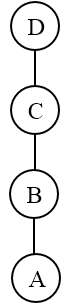
\includegraphics[scale = 1]{images/palm-aggregation-tree.png}
		\caption{Palm Shaped Aggregation Tree}
		\label{fig:Palm aggregation tree}
	\end{figure}
	While creating the commitment tree $A$ creates its data-item $A_{0}$ according to Equation \ref{eq:data-item}.
	$A$ sends only one data-item to $B$ therefore $A$'s payload ($A_{pay}$), transmit-payload ($A_{\tau}$) are given as follows:
	\begin{equation*}
		A_{pay} =\ <A_{0}, \textsf{Sign}_{\sk_{A}}(A_{0}), \textsf{Sign}_{\sk_{A}}(A_{\tau}) >\ where\ A_{\tau} =\ < A_{0} > 
	\end{equation*}
	The sensor node $C$'s payload is shown in Figure \ref{fig:Commitment payload of C}.
	The commitment tree generation process is described in the later sections. 
	The sensor node $C$ sends two data-items to $D$ therefore $C$'s payload ($C_{pay}$), transmit-payload ($C_{\tau}$) are given as follows:
	\begin{equation*}
		 	C_{pay} =\ <C_{0}, \textsf{Sign}_{\sk_{C}}(C_{0}), B_{1}, \textsf{Sign}_{\sk_{C}}(B_{1}), \textsf{Sign}_{\sk_{C}}(C_{\tau}) >\ where\ C_{\tau} =\ <B_{1}\ ||\ C_{0}>
	\end{equation*}

	\begin{figure}[h!]
		\centering
		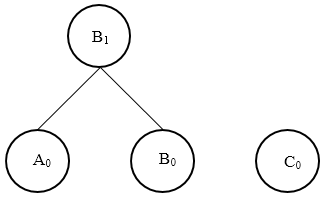
\includegraphics[scale = 1]{images/commitment-payload-of-C.png}
		\caption{Commitment Payload of Sensor Node $C$}
		\label{fig:Commitment payload of C}
	\end{figure}
	The verification of the received signatures in the payload is done by the parent node in the same way described in Section \ref{subsection:Signing and Verification of the Data-Item}.

	\subsection{Security Benefits}
		As described in Section \ref{subsec:security benefits of signing the data-item}, the signature of the transmit-payload $\textsf{Sign}_{S_{S}}(S_{\tau})$ assures the integrity and authentication of the transmit-payload $S_{\tau}$.
		In addition to that, the signature of the transmit-payload is like the signature for the transmission.
		To the sender, it assures that it is sending only the data-items included in the signature of the transmit-payload.
		Further, it establish that none of the data-items gets added or remove from the transmit-payload during the transmission. 
		To the receiver, it assures that it receives all the data-items included in the signature of the transmit-payload and none of the data-items were stranded or added additionally to the payload of its child.
		For example, the signature on the $C$'s transmit-payload $\textsf{Sign}_{\sk_{C}}(C_{\tau})$ assures that the sensor node $C$ sent only two data-items $C_{0},B_{1}$ in its payload.
		It also establishes that none of the data-items in its payload have been left stranded.
		% It is true for the sensor node $A$.
		As we said, it's like the signature for the transmission.

\section{Key Differences}

	In SHIA, all the leaf nodes in the aggregation tree send only their respective data-items to the parent in the aggregation tree.
	In our approach, all the leaf nodes send the data-item, the signature of the data-item and the signature of the transmit-payload to their parent node in the aggregation tree. 
	The child node sends its certificate as well if the parent node does not have it in its memory already.

	In SHIA, the parent node proceeds with the aggregation process without verifying the received data-items.
	In our protocol, the parent node verifies the received signature using the the verification algorithm.
	It proceeds with the aggregation only if all the signatures are verified true.

	In SHIA, the trusted base station verifies the final received data-items.
	And upon detecting the malicious activity in the network, the base station raises an alarm. 
	The base station does not do anything to detect malicious node responsible for the malicious activity.
	In our approach, upon detecting the malicious activity the base station interacts with several relevant nodes in the network to trace down the malicious node.
	Also, the base station issues the certificate to the sensor nodes in the network.
	
	\subsection{Bandwidth}
	
	% \textcolor{red}{Might need refactoring}
	According to Definition \ref{def:data-item}, the typical size of the data-item packet is $400$ bits as shown below.
	\begin{table}[!htb]	
  		\caption{Data-Item Size}
  		\centering
		\begin{tabular}{ | l | l | l | l |}
			\hline
			ID & COUNT & VALUE & COMMITMENT \\
			\hline
			20 bits & 21 bits & 20 bits & 256 bits\\
			\hline
		\end{tabular}
  	\end{table}
	If one uses Elliptic Curve Digital Signature Algorithm (ECDSA) then the size of signature is $500$ bits \cite{ecdsa2009186}.
	And the certificate size is $1500$ bits.
	So, at max we have to send additional $2000$ bits with the data-item.
	We think it is worthwhile to send these additional bits.
	Because of all the security benefits we gain from it. 
	\textbf{Note:} The packets size are close approximate to the actual packet size. 
	The actual packet size may differ based on the implementation.

\section{Two Ways of Forwarding Payload}	
	
	As described in the previous sections, we send the data-items with their signature along with the signature of the transmit-payload while creating the commitment tree.
	Here, we describe two different approaches to send the signatures in the aggregation tree hierarchy based on the two different ways of signing the data-items.
	To demonstrate two approaches we use the aggregation tree shown in Figure \ref{fig:Palm aggregation tree} and the payload of the sensor node $C$ shown in Figure \ref{fig:Commitment payload of C}.
	In both the approaches, the sensor node $C$ sends all the data-items in its payload with their respective signatures to its parent sensor node $D$ along with the signature of its transmit-payload $C_{\tau}$.

	In the first approach, $C$ verifies $\textsf{Sign}_{\sk_{B}}(B_{1})$ and sends it to $D$ without any modifications as follows:
	
	\begin{footnotesize}
		\begin{equation}	
			\begin{array}{l}
				C_{pay} =\ <C_{0},\textsf{Sign}_{\sk_{C}}(C_{0}),B_{1},\textcolor{red}{\textsf{Sign}_{\sk_{B}}(B_{1})}, \textsf{Sign}_{\sk_{C}}(C_{\tau})>\ where\ C_{\tau} = <C_{0} || B_{1}>\\
				C_{0} =\ <C_{id}, 1, C_{value}, H(N||1||C_{value})>\\
				B_{1} =\ <B_{id}, 2, B_{1value}, H(N||2||B_{1value}||A_{0}||B_{0})>;\ B_{1value} =\ B_{value} + A_{value}
			\end{array}
			\label{eq:forwarding-payload-without-resigning}
		\end{equation}
	\end{footnotesize}

	% The sensor node $C$ has two data-items $C_{0},B_{1}$ in its payload. 
	The sensor node $C$ sends three signatures $\textsf{Sign}_{\sk_{B}}(B_{1})$, $\textsf{Sign}_{\sk_{C}}(C_{0}) $ and $\textsf{Sign}_{\sk_{C}}(C_{\tau})$ to its parent $D$.
	It requires the parent node $D$ to know the public key of the sensor nodes $C$ and $B$, hence two certificates.

	In the second approach, the sensor node $C$ can verify the $\textsf{Sign}_{\sk_{B}}(B_{1})$ then remove the old signature and creates new signature $\textsf{Sign}_{\sk_{C}}(B_{1})$ and sends to $D$ as follows:

	\begin{footnotesize}
		\begin{equation}	
			\begin{array}{l}
				C_{pay} =\ <C_{0},\textsf{Sign}_{\sk_{C}}(C_{0}),B_{1},\textcolor{red}{\textsf{Sign}_{\sk_{C}}(B_{1})}, \textsf{Sign}_{\sk_{C}}(C_{\tau})>\ where\ C_{\tau} = <C_{0} || B_{1}>\\
				% C_{0} =\ <C_{id}, 1, C_{value}, H(N||1||C_{value})>\\
				% B_{1} =\ <B_{id}, 2, B_{1value}, H(N||2||B_{1value}||A_{0}||B_{0})>\\
			\end{array}
			\label{eq:forwarding-payload-with-resigning}
		\end{equation}
	\end{footnotesize}
	
	The sensor node $C$ sends three signatures $\textsf{Sign}_{\sk_{C}}(B_{1})$, $\textsf{Sign}_{\sk_{C}}(C_{0}) $ and $\textsf{Sign}_{\sk_{C}}(C_{\tau})$ to its parent $D$.
	But all the signatures are signed by the sensor node $C$, it requires the parent node $D$ to know the public key of only the sensor node $C$, hence $D$ need to know only one certificate.

	To give an analogy with a real world application, consider the following example.
	Suppose, one want to buy a diamond from the local diamond retailer.
	Some Diamonds are expensive commodity, so the end customer wants to verify its authenticity and integrity before purchasing.
	Now, suppose the diamond was created by the manufacturer in Africa, it was sold to a national wholesaler in the United States. 
	The national wholesaler sells it to the state level reseller and he sells it to the city or county level retailer from whom the customer purchases the diamond.

	One approach to verify the authenticity of the commodity is to make each entity in the supply chain to verify all the signatures on the received entity and sign on top of it.
	And then forward the commodity with all the signatures to the next entity in the supply chain.
	The next entity repeats the same procedure.
	Hence, any entity in the supply chain need to verify the signatures of all its descendants in the supply chain.
	In our example, it means to make the manufacturer from Africa signs the diamond and sells the signed diamond and sends the certificate to the national level wholesaler in United States.
	The national level wholesaler in United States verifies the signature from the manufacturer using manufacturer's certificate.
	Then he adds his signature and certificate, and sells the diamond signed with two signatures and two certificates to the state level reseller.
	The state level reseller verifies both the signatures on the diamond using the respective certificates.
	Then they add their signature and send their certificate, and sells the diamond singed with three signatures and three certificates to the city level retailer. 
	The city level retailer does the same thing before selling the diamond to the end customer.
	In the end, the customer needs to verify all four signatures, using the respective certificates.

	% Note: that the same diamond now has been signed by four different entities. And the end customer need to know the certificate of all four parties to verify all those signatures.

	An alternative approach to verify the authenticity of the commodity is to make each entity in the supply chain verify the signature, throw away the old signature, and then add its own signature on it. 
	It means the next entity in the supply chain need to verify only a single signature.
	The next entity repeats the same procedure.
	Hence, any entity in the supply chain need to verify the signature of only its direct peer in the supply chain. 
	In our example, it means to make the manufacturer from Africa signs the diamond and sells the signed diamond with his certificate to the national level wholesaler in United States.
	The national level wholesaler in United States verifies the signature from the manufacturer using the manufacturer's certificate.
	Then he removes the signature of the manufacturer, adds his own signature and certificate, and sells the diamond signed with one signature and one certificate to the state level reseller.
	The state level reseller verifies only the signature from the wholesaler using the wholesaler's certificate.
	Then they remove the signature of the wholesaler, adds their own signature and certificate, and sells the diamond signed with one signature and one certificate to the city level retailer.
	The city level retailer does the same thing before selling the diamond to the end customer.
	In the end, the customer needs to verify only one signature of the city level retailer using retailer's certificate.
	This approach requires very few number of certificates overall in the supply chain.

	We call these two approaches \textbf{Forwarding signatures without resigning the data-items (FSwoRD)}, \textbf{Forwarding signatures with resigning the data-items (FSwRD)} as shown in Equations \ref{eq:forwarding-payload-without-resigning} and \ref{eq:forwarding-payload-with-resigning} respectively.
	Both the approaches have their pros and cons and the perfect approach depends heavily on the application.
	The various aspects of both the approaches for sensor nodes are discussed in the following sections.

\chapter{Our protocol with resigning approach }
	In this chapter, we describe the entire protocol from the commitment tree generation to the result checking with resigning the data-item approach.

\section{Query Dissemination}
	The commitment tree generation process begins with the query dissemination.
	It is similar to the process described in section \ref{sec:query-dissemination}.

\section{Commitment Tree Generation}
	For the given aggregation tree the commitment forest is built as follows.
	The commitment tree generation begins from the sensor nodes with the highest depth (leaf nodes) in the aggregation tree.
	Leaf sensor nodes in the aggregation tree create their leaf vertex by creating data-items, signatures of those data-items and signature of the \textcolor{red}{transmit-payload} according to Equation \ref{eq:data-item}, \ref{eq:sign-data-item}, \ref{eq:signing-payload} respectively.
	And then send the payload to their parents in the aggregation tree.	
	Each internal sensor node in the aggregation tree also creates their leaf vertex.
	In addition, internal sensor node receives the data-items with the signatures of those data-items and the signature of the \textcolor{red}{transmit-payload} from each of its children which creates the forest for the internal sensor node.
	For all of its children, internal node first verifies the payload signature and then data-item signatures for one children at a time.
	Once internal node verifies all the received signatures, it merges all the data-items in its forest with same count value.
	Note that we can determine the height of the commitment tree from the count value.
	Suppose internal sensor node $I$ has to merge $i$ data-items $D_{1}$, $D_{2}$, $\dotsc$, $D_{i}$ in its forest.
	First, $I$ verifies all the received payload signatures.
	Then $I$ verifies the received signatures $Sign(D_{1})$, $Sign(D_{2})$, $\dotsc$, $Sign(D_{i})$.
	Once verified, $I$ starts merging the data-items as follows.
	Let $c$ be the smallest count value in $I$'s forest.
	The sensor node $I$ finds two data-items $D_{1},D_{2}$ in its forest with the same count value $c$ and merges them into a new data-item with the count of $c+1$ as shown in Figure \ref{fig:increase-height}.
	\begin{figure}[h!]
		% \centering
		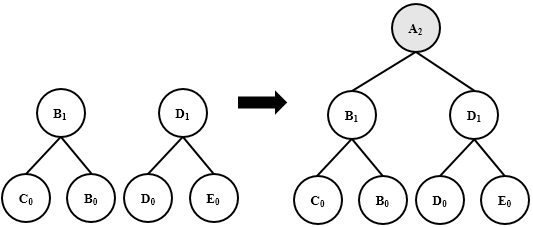
\includegraphics[width=6in]{images/increase-height.png}
		\caption{$A$ has $B_{1}, C_{1}$ in his forest and aggregates those two trees and creates $A_{2}$.}
		\label{fig:increase-height}
	\end{figure}
	It repeats the process until no two data-items in its forest have the same count value.	
	
	We demonstrate the commitment tree generation process for the aggregation tree shown in Figure \ref{fig:Aggregation-tree-1}.
		\begin{figure}[h!]
			\centering
			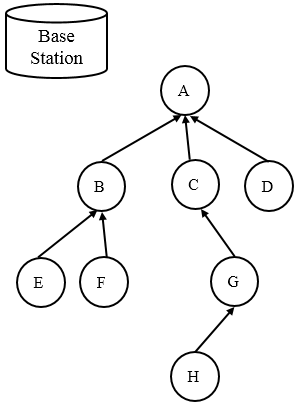
\includegraphics[scale=1]{images/aggregation-tree-1.png}
			\caption{Aggregation Tree.}
			\label{fig:Aggregation-tree-1}
		\end{figure}
		In this example, $A$ has three children. $A$ receives one payload from each of its children which creates $A$'s forest.
		After verifying all the signatures from its forest, $A$ uses the data-items in its forest to create its payload, which is sent to the base station.
		First, we describe the payload generation process of $B,C,D$ and then for $A$.

		The sensor node $B$ creates its payload from its forest. 
		It's forest consists of payloads received from $E,F$.
		The leaf sensor nodes $E,F$ creates their payloads according to Equation \ref{eq:signing-payload} as follows:
		% \begin{figure}[h!]
		% 	\centering
		% 	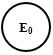
\includegraphics{images/e-payload.png}
		% 	\caption{E's payload}
		% 	\label{fig:e-payload}
		% \end{figure}
		\begin{equation}
			\begin{array}{l}
			E_{p} =\ <E_{0}, \textsf{Sign}_{S_{E}}(E_{0}), \textsf{Sign}_{S_{E}}(E_{\tau}) >\ where\ E_{\tau} =\ <E_{0}>\\
			E_{0} =\ <E_{id}, 1, E_{value}, H(N||1||E_{value})>
			\end{array}
		\end{equation}
		% \begin{figure}[h!]
		% 	\centering
		% 	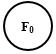
\includegraphics{images/f-payload.png}
		% 	\caption{F's payload}
		% 	\label{fig:f-payload}
		% \end{figure}
		\begin{equation}
			\begin{array}{l}
				F_{p} =\ <F_{0}, \textsf{Sign}_{S_{F}}(F_{0}), \textsf{Sign}_{S_{F}}(F{\tau}) >\ where\ F_{\tau} =\ <F_{0}>\\
				F_{0} =\ <F_{id}, 1, F_{value}, H(N||1||F_{value})>
			\end{array}
		\end{equation}
		$B$ receives $E_{p},F_{p}$ from $E,F$ respectively. 
		$B$ verifies all the signatures in the received payloads.
		Then it creates $B_{0}$.
		Now, $B$ has $B_{0},E_{0},F_{0}$ in its forest as shown in Figure \ref{fig:b-forest-payload}. 
		As all the data-items have the same count value, $B$ has an option which two to aggregate.
		$B$ aggregates $E_{0},F_{0}$ and creates $B_{1}$.
		After creating $B_{1}$ none of the data-items have the same count value. 
		So, $B$ creates its payload $B_{p}$ and sends it to $A$ as follows:
		\begin{equation}
			\begin{array}{l}
				B_{p} =\ < B_{0}, \textsf{Sign}_{S_{B}}(B_{0}), B_{1}, \textsf{Sign}_{S_{B}}(B_{1}), \textsf{Sign}_{S_{B}}(B_{\tau}) >\ where\ B_{\tau} =\ <B_{0} || B_{1}>\\
				B_{1} =\ < B_{id}, 2, B_{1value}, H(N||2||B_{1value}||E_{0}||F_{0})>;\ B_{1value} = E_{value} + F_{value} \\
				B_{0} =\ <B_{id}, 1, B_{value}, H(N||1||B_{value})>
			\end{array}
			\label{eq:b-payload}
		\end{equation}
		\begin{figure}[h!]
			\centering
			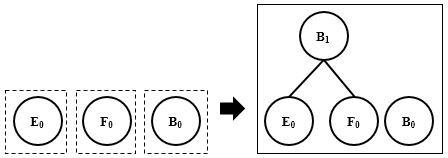
\includegraphics[scale=1]{images/b-forest-payload.png}
			\caption{$B$'s forest aggregation creating its payload.
			 				Each dashed-line box shows forest and solid-line box shows payload of the respective sensor node.}
			\label{fig:b-forest-payload}
		\end{figure}

		In similar way $C$ receives $G_{p}$ from $G$ defined as follows:
		\begin{equation}
			\begin{array}{l}
				G_{p} =\ <G_{1},\textcolor{red}{\textsf{Sign}_{S_{G}}(G_{1})}, \textsf{Sign}_{S_{G}}(G_{\tau})>\ where\ G_{\tau} =\ <G_{0} || H_{0}>\\
				G_{1} =\ < G_{id}, 2, G_{1value}, H(N||2||G_{1value}||G_{0}||H_{0})>;\ G_{1value} = G_{value} + H_{value} \\
				G_{0} =\ <G_{id}, 1, G_{value}, H(N||1||G_{value})>\\
				H_{0} =\ <H_{id}, 1, H_{value}, H(N||1||H_{value})>
			\end{array}
		\end{equation}
		$C$ verifies all the signatures in the received payload $G_{p}$ and creates $C_{0}$.
		Now, $C$ has $C_{0},G_{1}$ in its forest as shown in Figure \ref{fig:c-forest-payload}. 
		As none of the data-items have the same count value, $C$ does not aggregate.
		But $C$ removes the old signature $G_{1}$ and put its own signature on $G_{1}$.
		So, $C$ creates its payload $C_{p}$ and sends it to $A$ as follows:
		\begin{figure}[h!]
			\centering
			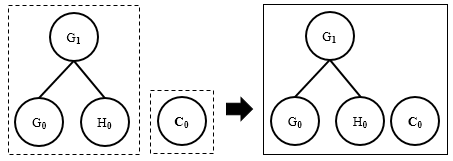
\includegraphics[scale=1]{images/c-forest-payload.png}
			\caption{$C$'s forest aggregation creating its payload.}
			\label{fig:c-forest-payload}
		\end{figure}
		\begin{equation}
			\begin{array}{l}
				C_{p} =\ <C_{0},\textsf{Sign}_{S_{C}}(C_{0}),G_{1},\textcolor{red}{\textsf{Sign}_{S_{C}}(G_{1})}, \textsf{Sign}_{S_{C}}(C_{\tau})>\ where\ C_{\tau} =\ <C_{0} || G_{1}>\\
				C_{0} =\ <C_{id}, 1, C_{value}, H(N||1||C_{value})>
			\end{array}
			\label{eq:c-payload}
		\end{equation}

		The sensor node $D$ creates its payload and sends it to $A$ as follows:
		\begin{equation}
			\begin{array}{l}
				D_{p} =\ <D_{0}, \textsf{Sign}_{S_{D}}(D_{0}), \textsf{Sign}_{S_{D}}(D_{\tau})>;\ where\ D_{\tau} =\ <D_{0}>\\
				D_{0} =\ <D_{id},1,D_{value},H(N||1||D_{value})>
			\end{array}
			\label{eq:d-payload}
		\end{equation}

		The root node of the aggregation tree $A$ receives $B_{p}, C_{p}, D_{p}$
		% Equations \ref{eq:b-payload},\ref{eq:c-payload},\ref{eq:d-payload} 
		from $B,C,D$ respectively.
		$A$ verifies all the signatures in the received payloads and creates $A_{0}$.
		$A$ has $G_{1},C_{0},B_{1},B_{0},D_{0},A_{0}$ in its forest as shown in Figure \ref{fig:a-forest}.
		\begin{figure}[h!]
			\centering
			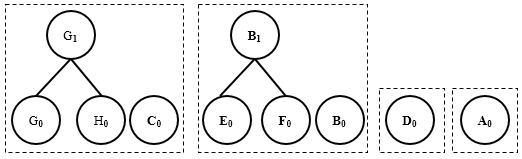
\includegraphics[scale=1]{images/a-forest.png}
			\caption{$A$'s forest: $A$ receives three payloads from $C,B,D$ and creates $A_{0}$}
			\label{fig:a-forest}
		\end{figure}
		\begin{figure}[h!]
			\centering
			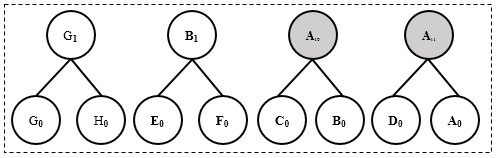
\includegraphics[scale=1]{images/a-forest-first-merge.png}
			\caption{$A$'s forest after first merge}
			\label{fig:a-forest-first-merge}
		\end{figure}
		\begin{figure}[h!]
			\centering
			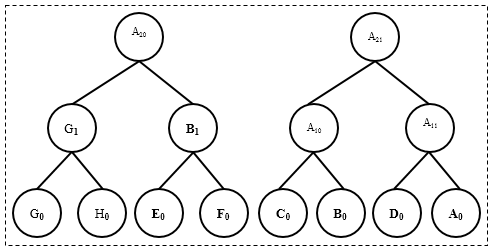
\includegraphics[scale=1]{images/a-forest-second-merge.png}
			\caption{$A$'s forest after second merge}
			\label{fig:a-forest-second-merge}
		\end{figure}
		$A$ has four data-items with count value of $1$.
		In the first merge, $A$ aggregates those data-items and creates $A_{10},A_{11}$ as shown in Figure \ref{fig:a-forest-first-merge}.
		Now, $A$ has four data-items with count value of $2$.
		In the second merge, $A$ aggregates those data-items and creates $A_{20},A_{21}$ as shown in Figure \ref{fig:a-forest-second-merge}.
		Finally, $A$ has two data-items with count value of $4$.
		In the final merge, $A$ aggregates those data-items and creates $A_{3}$ as shown in Figure \ref{fig:a-payload}.
		Then $A$ creates payload and sends it to the base station as follows:
		\begin{equation}
			\begin{array}{l}
				A_{p} =\ <A_{3},\textsf{Sign}_{S_{A}}(A_{3}),\textsf{Sign}_{S_{A}}(A_{\tau})>\ where\ A_{\tau} =\ <A_{3}>\\
				A_{3} =\ <A_{id}, 8, A_{3value}, H(N||8||A_{3value}||A_{20}||A_{21})>;\ A_{3value} =\ A_{20value} + A_{21value}\\
				A_{20} =\ <A_{id},4,A_{20value},H(N||4||A_{20value}||G_{1}||B_{1})>;\ A_{20value} =\ G_{1value} + B_{1value}\\ 
				A_{21} =\ <A_{id},4,A_{21value},H(N||4||A_{21value}||A_{10}||A_{11})>;\ A_{21value} =\ A_{10value} + A_{11value}\\ 
				A_{10} =\ <A_{id},2,A_{10value},H(N||2||A_{10value}||B_{0}||C_{0})>;\ A_{10value} =\ B_{value} + C_{value}\\
				A_{11} =\ <A_{id},2,A_{11value},H(N||2||A_{11value}||D_{0}||A_{0})>;\ A_{11value} =\ D_{value} + A_{value}\\
				A_{0} =\ <A_{id},1,A_{value},H(N||1||A_{value})>
			\end{array}
		\end{equation}
		\begin{figure}[h!]
			\centering
			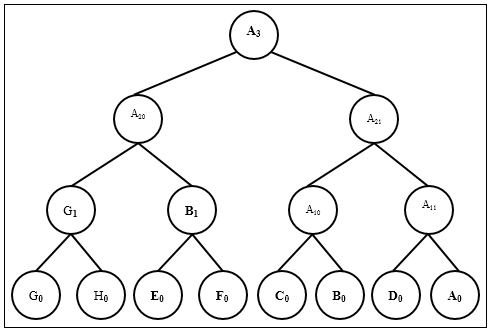
\includegraphics[scale=1]{images/a-payload.png}
			\caption{$A$'s payload : $A$ sends this to the base station.}
			\label{fig:a-payload}
		\end{figure}

				% \begin{figure}[h!]
				% 	\centering
				% 	% 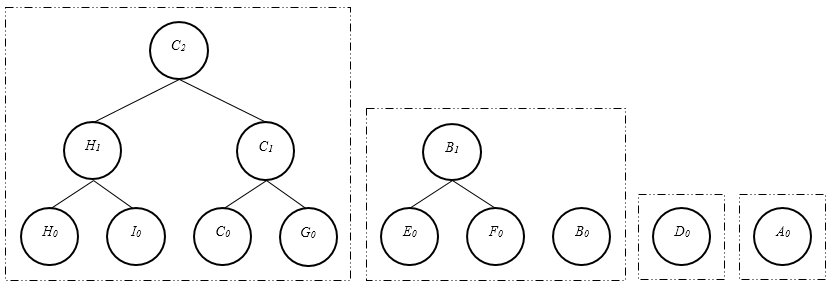
\includegraphics[width=6in]{images/commitment-tree-example-1.png}\\
				% 	\caption{$A$ receives $C_{2}$ from $C$, $(B_{1},B_{0})$ from $B$, $D_{0}$ from $D$ and generates $A_{0}$. The commitment payload received from a given sensor node is indicated by dashed-line box.}
				% 	\label{fig:commitment-tree-example-1}
				% \end{figure}
				% \begin{equation}
				% 	\begin{array}{l}
				% 		A_{0} = <A_{id}, 1, A_{value}, H(N||1||A_{value})>; \textsf{Sign}_{S_{A}}(A_{0}) \\
				% 		D_{0} = <D_{id}, 1, D_{value}, H(N||1||D_{value})>; \textsf{Sign}_{S_{D}}(D_{0})\\
				% 		B_{0} = <B_{id}, 1, B_{value}, H(N||1||B_{value})>; \textsf{Sign}_{S_{B}}(B_{0})\\
				% 		B_{1} = <B_{id}, 2, B_{value}, H(N||2||B_{value}||E_{0}||F_{0})>; \textsf{Sign}_{S_{B}}(B_{1})\\
				% 		\textcolor{red}{\textsf{Sign}_{S_{B}}(B_{0} || B_{1}), benefits}\\
				% 		C_{2} = <C_{id}, 4, C_{value}, H(N||4||C_{value})||H_{1}||C_{1})>; \textsf{Sign}_{S_{C}}(C_{2})\\
				% 		\end{array}
				% \end{equation}

				% \begin{figure}[h!]
				% 	\centering
				% 	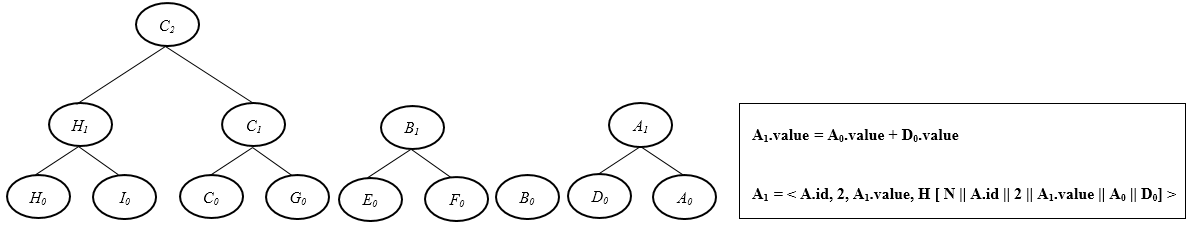
\includegraphics[width=6in]{images/commitment-tree-example-2.png}\\
				% 	\caption{First Merge: $A_{1}$ vertex created by A.}
				% 	\label{fig:commitment-tree-example-2}
				% \end{figure}

				% \begin{equation}
				% 	\begin{array}{l}
				% A_{1} = <A_{id}, 2, A_{1value}, H(N||2||A_{1value}||A_{0}||D_{0})>; \textsf{Sign}_{S_{A}}(A_{1})\\
				% where\  A_{1value} = A_{value} + D_{value} \\
				% 	\end{array}	
				% \end{equation}
				% \begin{figure}[h!]
				% 	\centering
				% 	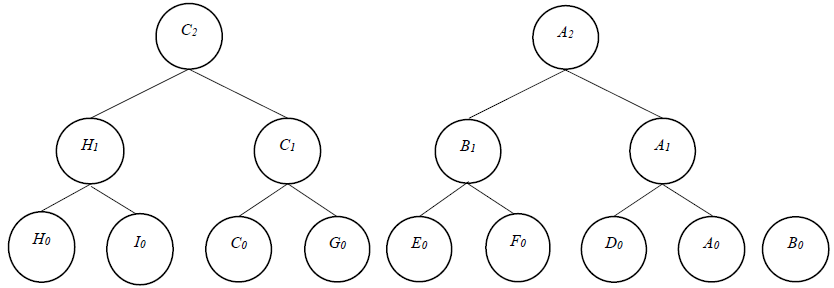
\includegraphics[width=\textwidth]{images/commitment-tree-example-3.png}\\
				% 	\caption{Second Merge: $A_{2}$ vertex created by A.}
				% 	\label{fig:commitment-tree-example-3}
				% \end{figure}
				% \begin{equation}
				% 	\begin{array}{l}
				% 		A_{2} = <A_{id}, 4, A_{2value}, H(N||4||A_{2value}||B_{1}||A_{1}) >; \textsf{Sign}_{S_{A}}(A_{2})\\
				% 		where\  A_{2value} = B_{1value} + A_{1value} \\
				% 	\end{array}
				% \end{equation}
				% \begin{figure}[h!]
				% 	\centering
				% 	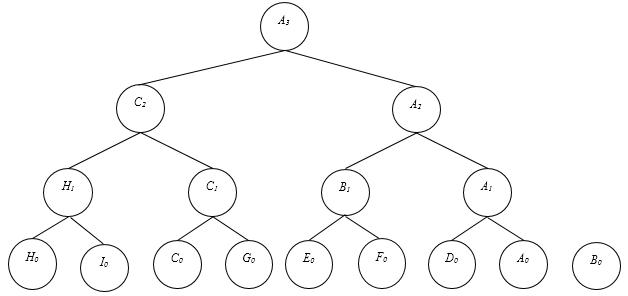
\includegraphics[width=6in]{images/commitment-tree-example-4.png}\\
				% 	\caption{Third Merge: $A_{3}$ vertex created by A.}
				% 	\label{fig:commitment-tree-example-4}
				% \end{figure}
				% \begin{equation}
				% 	\begin{array}{l}
				% 		A_{3} = <A_{id},8, A_{3value},H(N||8||A_{3value}||C_{2}||A_{2})>; \textsf{Sign}_{S_{A}}(A_{3})\\
				% 		where\ A_{3value} = A_{2value} + C_{2value}
				% 	\end{array}
				% \end{equation}

	Once the base station receives the payload from the root of the aggregation tree, it verifies all the signatures in the payload.
	In the previous example the base station receives $A_{p}$ from the sensor node $A$.
	It verifies the signatures $\textsf{Sign}_{S_{A}}(A_{3})$, $\textsf{Sign}_{S_{A}}(A_{\tau})$ in the received payload.	 
	If the base station verifies all the signatures to true it initiates the result checking phase.

\section{Result checking by the sensor nodes}
	The purpose of the result checking phase is to enable all the sensor nodes to verify their individual contributions to the final aggregate value.
	If there is any inconsistency in the aggregation process then with the help of the base station, trace down the node responsible for causing the inconsistency in the aggregation process.

	\subsection{Dissemination Final Payload}
		After the base station has received the payloads of the root node of the aggregation tree, the base station sends each of the data-items in the payload to the entire sensor network using authenticated broadcast.
		We use authenticated broadcast allows the sensor nodes to verify that this data-items are coming from the base station.
		In our previous example, the base station receives only one data-item $A_{3}$ in the payload received from $A$.
		In that case, the base station's payload $\textsf{B}_{p}$ is given as follows:
 		\begin{equation}
			\textsf{B}_{p} =\ <A_{3}, \textsf{Sign}_{S_{\textsf{B}}}(A_{3}), \textsf{Sign}_{S_{\textsf{B}}}(\textsf{B}_{\tau})>\ where\ \textsf{B}_{\tau} =\ <A_{3}>
		\end{equation}

	\subsection{Dissemination of Off-Path Values}
		To enable verification each sensor node must receive all of its off-path values.
		The off-path values of the sensor nodes can be determined according to the Definition \ref{def:off-path}.
		
		Each internal vertex $t$ in the commitment tree has two children $u1$ and $u2$. 
		To disseminate off-path values, $t$ sends the data-item of $u1$ to $u2$, and vice-versa ($t$ also attaches relevant information tagging $u1$ as the right child and $u2$ as the left child) along with the signatures of the data-item and the signature of the transmit-payload.
		In our previous example, internal vertex $A_{10}$ as shown in Figure \ref{fig:a-payload} has two children $C_{0},B_{0}$.
		$A_{10}$ sends the following off-path values as follows to $C, B$ respectively.
		\begin{equation}
			\begin{array}{l}
			<B_{0}, \textsf{Sign}_{S_{A}}(B_{0}),\textsf{Sign}_{S_{A}}(A_{10\tau})>\ where\ A_{10\tau} =\ <B_{0}>\\
			<C_{0}, \textsf{Sign}_{S_{A}}(C_{0}),\textsf{Sign}_{S_{A}}(A_{10\tau})>\ where\ A_{10\tau} =\ <C_{0}>
			\end{array}
		\end{equation}
		An internal vertex $t$ receives data-items with their respective signatures from its parent. 
		It verifies the signatures of the data-items and then sends data-items (and left/right tags) to both of its children.
		Continuing the previous example, internal vertex $A_{10}$ receives $A_{11}, A_{20}$ form its parent $A_{21}$.
		$A_{10}$ sends the following off-path values as follows to $C, B$ respectively.
		\begin{equation}
			\begin{array}{l}
			<B_{0}, \textsf{Sign}_{S_{A}}(B_{0}),A_{11},\textsf{Sign}_{S_{A}}(A_{11}),A_{20},\textsf{Sign}_{S_{A}}(A_{20}),\textsf{Sign}_{S_{A}}(A_{10\tau})>\\ 
				where\  A_{10\tau} =\ <B_{0}||A_{11}||A_{20}>\\
			<C_{0}, \textsf{Sign}_{S_{A}}(C_{0}),A_{11},\textsf{Sign}_{S_{A}}(A_{11}),A_{20},\textsf{Sign}_{S_{A}}(A_{20}),\textsf{Sign}_{S_{A}}(A_{10\tau})>\\ 
				where\  A_{10\tau} =\ <C_{0}||A_{11}||A_{20}>
			\end{array}
		\end{equation}

	\subsection{verification of inclusion}
	\subsection{collection of authentication codes}

\section{Result checking by the base station}
	\subsection{verification of authentication codes}
		\label{sec:verficiation-of-authentication-codes}
		The authentication codes for sensor node $s$, with either positive or negative acknowledgment message, are defined as follows:
		\begin{equation}
			MAC_{K_{s}}(N\ ||\ \textit{ACK})
		\end{equation}
		\begin{equation}
			MAC_{K_{s}}(N\ ||\ \textit{NACK})
		\end{equation}
		$K_{s}$ is the key that $s$ shares with the base station;
		$\textit{ACK}$, $\textit{NACK}$ are special messages for positive and negative acknowledgment respectively.
		The authentication code with $\textit{ACK}$ message is sent by the sensor node if it verifies its contribution correctly to the root commitment value during the 
		\textit{verification of inclusion} phase and vice versa.
		
		To verify that every sensor node has sent its authentication code with \ack, the base station computes the $\Delta_{ack}$ as follows:
		\begin{equation}
			\displaystyle{\Delta_{ack} = \bigoplus_{i = 1}^n MAC_{K_{i}}(N || ACK) }
		\end{equation}
		The base station can compute $\Delta_{ack}$ as it knows $K_{s}$\ for each sensor node $s$.
		Then it compares the computed $\Delta_{ack}$\ with the received root authentication code $\Delta_{root}$\ from the root of the aggregation tree. 
		If those two codes match then it accepts the aggregated value or else it proceeds further to find an adversary. 

		To detect an adversary, the base station needs to identify which nodes in the aggregation tree sent its authentication codes with \nack\ during the verification of inclusion phase.
		The node who sent authentication code with \nack\ during the verification of inclusion phase is called a \complainer. 
		We claim that if there is a single complainer in the aggregation tree during the verification of inclusion phase then the base station can find the complainer in linear time.
		To find a complainer, the base station computes the complainer code $c$.
		\begin{equation}\label{eq:complainer}
			c := \Delta_{root} \oplus \Delta_{ack}
		\end{equation}
		Then it computes the complainer code $c_{i}$\ for all node $i = 1, 2, \dotsc, n$. 
		\begin{equation}\label{eq:caomplainer-node}
			c_{i} := MAC_{K_{i}}(N\ ||\ \textit{ACK}) \oplus MAC_{K_{i}}(N\ ||\ \textit{NACK})
		\end{equation}
		Then it compares $c$\ with all $c_{i}$\ one at a time. 
		The matching code indicates the complainer node.
		The base station needs to do $n \choose 1$\ calculations according to Equation \ref{eq:caomplainer-node} and same number of comparisons to find a complainer in the aggregation tree. 
		Hence, the base station can find a single complainer in linear time.
		\begin{exmp} If there are four nodes ${s_{1},s_{2},s_{3},s_{4}}$ in an aggregation tree and their authentication codes with \ack, \nack\ message in the binary format are defined below.\\
			$\mac_{K_{1}}(N\ ||\ \ack)$ = $(1001)_{2}\ ;\ $
			$\mac_{K_{1}}(N\ ||\ \nack)$ = $(1101)_{2}$\\
			$\mac_{K_{2}}(N\ ||\ \ack)$ = $(0110)_{2}\ ;\ $
			$\mac_{K_{2}}(N\ ||\ \nack)$ = $(1111)_{2}$\\	
			$\mac_{K_{3}}(N\ ||\ \ack)$ = $(0101)_{2}\ ;\ $
			$\mac_{K_{3}}(N\ ||\ \nack)$ = $(0111)_{2}$\\
			$\mac_{K_{4}}(N\ ||\ \ack)$ = $(0011)_{2}\ ;\ $
			$\mac_{K_{4}}(N\ ||\ \nack)$ = $(1110)_{2}$\\
			$\Delta_{root} = (0100)_{2}$\\
			$\Delta_{ack} = (1101)_{2}$\\
			$c_{1} = (0100)_{2}$, $c_{2} = (1001)_{2}$, $c_{3} = (0010)_{2}$, $c_{4} = (1101)_{2}$\ \\
			$c = (1101)_{2}$
			$c$ is equal to $c_{4}.$\\
			So, the base station identifies that the $s_{4}$\ complained, during verification of inclusion phase.\\ 
		\end{exmp}
		In general, to find $k$\ complainers the base station needs to do $ n \choose k$\ calculations and the same number of comparisons to find $k$\ complainers.
		
		\textcolor{red}{How XOR is negating the contribution of NACK.}
		\[ 
			\left( 
				\begin{array}{cccc}
					1 & 0 & 0 & 1 \\ 
					0 & 1 & 1 & 0 \\
					0 & 1 & 0 & 1 \\
					0 & 0 & 1 & 1 \\
					\hline
					1 & 0 & 0 & 1 
				\end{array}
			\right)
		%
			\left( 
				\begin{array}{cccc}
					1 & 1 & 0 & 1 \\ 
					1 & 1 & 1 & 1 \\
					0 & 1 & 1 & 1 \\
					1 & 1 & 1 & 0 \\
					\hline
					1 & 0 & 1 & 1 
				\end{array}
			\right)
		\]

		The base station receives the following:
		\[ 
			\left( 
				\begin{array}{cccc}
					1 & 0 & 0 & 1 \\ 
					0 & 1 & 1 & 0 \\
					0 & 1 & 0 & 1 \\
					1 & 1 & 1 & 0 \\
					\hline
					0 & 1 & 0 & 0 
				\end{array}
			\right)
		\]

		The base station does the following:

		\[
			\left( 
				\begin{array}{cccc cccc cccc cccc}
					1 & 0 & 0 & 1\ \vline\  0 & 1 & 1 & 0\ \vline\  0 & 1 & 0 & 1\ \vline\  0 & 0 & 1 & 1 \\
					1 & 1 & 0 & 1\ \vline\  1 & 1 & 1 & 1\ \vline\	0 & 1 & 1 & 1\ \vline\	1 & 1 & 1 & 0 \\ 
					\hline
					0 & 1 & 0 & 0\ \vline\ 1 & 0 & 0 & 1\ \vline\ 0 & 0 & 1 & 0\ \vline\ 1 & 1 & 0 & 1\\
				\end{array}
			\right)
		\]

		\[ 
			\left( 
				\begin{array}{cccc}
					1 & 0 & 0 & 1 \\ 
					0 & 1 & 0 & 0 \\
					\hline
					1 & 1 & 0 & 1 \\
				\end{array}
			\right)
		\]

		And concludes that node $4 $ is complaining.
	\newpage
	\subsection{Detect an adversary}
		\begin{algorithm}
		\caption{Pseudo algorithm to detect an adversary}
		\label{algo:detect-an-adversary}

			\begin{algorithmic}[1]

					\STATE $BS$ \ identifies all the complainer and creates $c = \{c_{1}, c_{2}, \dotsc, c_{n}\}$
					\FORALL {$N \in c$}

						\STATE $BS$\ asks $N$ to send data-items with its signature, sent during commitment tree generation phase
					
					\ENDFOR

					\STATE $BS$\ identifies possible adversary based on $c$ and creates $a = \{a_{1},a_{2},\dotsc,a_{n}\}$

					\FORALL {$A \in a$}

						\STATE $BS$\ asks $A$ to send data-items with its signature, received and sent by $A$ during commitment tree generation phase
						\STATE If needed $BS$\  asks the parent of $A$ to send data-items with its signature
			
					\ENDFOR

					\STATE $BS$\ determines the adversary based on the verification of signatures

			\end{algorithmic}
		\end{algorithm}

	\begin{theorem}
		%\emph{(Lagrange's Theorem)}
		\label{Commitment tree}
		Binary commitment tree is optimal in terms of verification as it requires minimum number of off-path values.
	\end{theorem}

	\begin{proof}
		Let us say $n$ is the number of leaves in the given commitment tree.

		$ \log _3( n ) = y $

		$ 3^y = n $

		$ \log_2( 3^y ) = \log_2( n ) $

		$ y * \log_2( 3 ) = \log_2( n ) $

		$ \log_3( n )*\log_2( 3 ) = \log_2( n ) $

		$ \log_3( n ) = \frac{ {\log _2 ( n )} }{{\log _2 ( 3 )}} $

		$ 2 * \log_3( n ) = [2 / \log_2( 3 ) ]* log_2( n ) = ( 1.2618 ) * log_2( n ) $

		$ 2 * log_3( n ) > log_2( n ) $ \\
		For the given binary commitment tree, each leaf vertex needs $\log_{2}(n)$ off-path values in the verification phase.
		The total off-path values needed in the given commitment tree is $n \cdot \log_{2}(n)$.\\
		For the given tertiary commitment tree, each leaf vertex needs $2 \cdot \log_{3}(n)$ off-path values in the verification phase.
		The total off-path values needed in given commitment tree is $2 \cdot n \cdot \log_{3}(n)$.

		Hence, in totality the binary commitment tree requires the minimum number of off-path values.
	\end{proof}

	\begin{theorem}
	\cite{chan2006secure}
	The Aggregate Commit with verification induces $O(\log^3 n)$ edge congestion. And $O(\delta\log^3 n)$ node congestion in the aggregation tree.
	\end{theorem}
	\begin{proof}
		While creating the commitment tree every sent message is at most $O(\log n)$ size.
		And while the off-path value dissemination step is the
	% dominating factor.
	% Consider an arbitrary edge in the commitment-tree between parent
	% vertex x and child vertex y. In the label dissemination step,
	% messages are only sent from parent to child in the commitment tree.
	% Hence the edge xy carries exactly the labels that y receives. From
	% Theorem 14, y receives O(logn) labels, hence the total number of
	% labels passing through xy is O(logn). Hence, the edge congestion
	% in the commitment tree is O(logn). Now consider an arbitrary aggregation
	% tree edge with parent node u and child node v. The child
	% node v presents (i.e., sends) at most logn commitment-tree vertices
	% to its parent u, and hence the edge uv is responsible for carrying
	% traffic on behalf of at most logn commitment-tree edges — these
	% are the edges incident on the commitment tree vertices that v presented
	% to u. Note that v may not be responsible for creating all
	% the vertices that it presents to u, but v is nonetheless responsible
	% for forwarding the messages down to the sensor nodes which created
	% those vertices. Since each edge in the commitment tree has
	% O(logn) congestion, and each edge in the aggregation tree carries
	% traffic for at most logn commitment-tree edges, the edge congestion
	% in the aggregation tree is O(log2 n). The node-congestion bound
	% of O(Δlog2 n) follows from the O(log2 n) edge congestion and the
	% definition of Δ as the greatest degree in the aggregation tree.
	\end{proof}


\section{Bandwidth Analysis}
	For any given sensor node's forest with $n$ leaf vertices, has at most $\log n$ data-items in its payload.
	It has at most $(\log n) +1$ signatures in its payload.
	The highest possible count value is $\log n$, as all the trees are binary. 

	An intermediate sensor node $S$ with $\beta$ descendants in the aggregation tree, has at most $\log(\beta+1)$ data-items with their respective $\log(\beta+1)$ signatures in its payload.
	$S$ might need to send its payload signature $Sign(S_{p})$.
	At max, $S$ has to send a payload with $\log(\beta+1)$ data-items and $\log(\beta+1) +1$ signatures to its parent in the aggregation tree.
	
	Hence, sending signatures of the data-items causes $O(\log \beta)$ bandwidth overhead for each node in the network, where $\beta$ is the number of descendants of the sensor node. 


\section{Performance Analysis}
	In addition to calculating its own data-items, all intermediate sensor nodes with $\beta$ descendants and $\zeta$ direct children need to do the following:
	\begin{itemize}
		\item To calculate and verify $O(\log \beta)$ signatures, creating $O(\log \beta)$ calculation overhead. 
		\item Needs sufficient memory to cache $O(\log \beta)$ certificates. 
		\item Needs enough memory to cache $\Omega(\zeta)$ certificates.
	\end{itemize}

	% Computation cost: Needs to calculate that many signatures. Needs to verify that many signatures.
	% Need to know that many certificates.

\section{Applications}
		The signature based aggregation scheme can be applied to do the \textbf{voting} in the network.
		And voting scheme can be used to solve many sensor network problems.
		For example, voting can be used to design the distributed algorithm for selecting a cluster head or node revocation system.
		In the voting scheme, following are the major security concerns: 
		\begin{itemize}
			\item The aggregate node needs to know that the vote is coming from the legit voter, no other voter is impersonating the vote of the legit voter.
			\item Only the intended aggregate node should be able to verify the vote.
			\item The aggregate node should not be able to tamper with the votes. 
			\item The aggregate node needs the proof that it aggregated the verified votes.
			\item The voter need the proof for which vote it sent to its aggregator.
		\end{itemize}
		For example, the base station wants to know the overall vote-count in the network.
		To do so, all the leaf nodes send their votes and the signature of their votes to their respective aggregate nodes in the network.
		The aggregate nodes receive votes with their signatures from all of their children voters.
		The aggregate nodes verify all the votes and count those votes.
		Then they forward the count and the signature of that count signed by the aggregate node to their respective parent in the aggregation tree.
		This process is repeated until the final count and its signature, is sent to the base station by the root of the aggregation tree.
				
\textbf{Node power level},
\textbf{Surveillance Application}

% \chapter{Notes}

\begin{itemize}
	\item Do we hash node's id in the commitment field of its data-item? NO
	\item Do we send the payload signature in case of Figure 5.4? YES
\end{itemize}

To do list:
\begin{itemize}
	% \item ch-3: signatures from 628; All PKI are not digital signatures capable.
	% \item ch-5: Clear goals of the protocol.
	% \item Review the writing.
	% \item ch-2: Add smooth transition to the security section.
	% \item ch-2: add more applications in section 2.1.
	% \item ch-4: change sign label
	% \item ch-4: Why SHIA does not have ID in their label? Why do you have ID? What benefits you get out of it?
	\item Cheating: Finish writing about detecting a cheater.
	\item ch-4: Image modifications. Update images with darker borders. Decrease width. Save word as pdf and then crop images
	\item Review the writing.

	\item 3. Discuss cheating, distributing off-path.  
	\item ch-6: Why don't you need signatures with off-path?
	\item ch-4: Advantages of signing the B's payload.

	\item ch-3: cite book for digital signatures

	\item ch-6: removing old signatures, and signing those again
	\item ch-6: equation for number of certificates needed in the network

\end{itemize}
% Summary and/or conclusions are optional but often used.
% The summary and/or conclusions often are the last
% major division(s) of the text.
% Reference: TM 32.
% CHANGE NEXT LINE?
%
%  summary.tex  2007-02-06  Mark Senn  http://www.ecn.purdue.edu/~mark
%

\chapter{Summary}

This is the summary chapter.


% Recommendations are optional.
% You may include recommendations as a major division if your
% subject matter and research dictate.
% Reference: TM 32.
% CHANGE NEXT LINE?
%
%  recommendations.tex  2007-02-06  Mark Senn  http://www.ecn.purdue.edu/~mark
%

\chapter{Recommendations}

Buy low.  Sell high.


% Bibliography is required if you consulted any outside references.
% Reference: TM 32.
%
%  bibliography.tex     June 3, 2002     Mark Senn
%
%  This is the bibliography for a simple, example thesis.
%

\bibliography{all}


% Appendices are optional.
% Appendices are not necessarily part of every thesis. Appendices are used
% for supplementary illustrative material, original data, computer programs,
% and other material not necessarily appropriate for inclusion within the
% text of your thesis. 
% Reference: TM 33.
% Use "\appendix" for one appendix or "\appendices" for more than one
% appendix.
% CHANGE NEXT 7 LINES?
%\appendices
%%
%  revised  demo-citations.tex  2011-09-02  Mark Senn  http://www.ecn.purdue.edu/~mark
%  created  demo-citations.tex  2007-03-21  Mark Senn  http://www.ecn.purdue.edu/~mark
%


\chapter{Demonstrate Citations}

%I typed

\begin{verbatim}
    
	\cite{Campdoop: Exploiting In-network Aggregation for Big Data Applications}
    %For \LaTeX\ answers I refer to
    %% note to self: {\em \LaTeX: A Document Preparation System\/}
    %\cite{Lamport:1994}
    %and then to
    %% note to self: {\em The \LaTeX\ Companion\/}
    %\cite{Goossens:1994}
    %or
    %% note to self: {\em A Guide to LaTeX\/} (1999)
    %\cite{Kopka:1999}.
   % % note to self: {\em A Guide to LaTeX\/} (1999)
    %\cite{Kopka:1999}
    %is an updated edition of the 1995 edition
    %\cite{Kopka:1995}.
\end{verbatim}

to get

\begin{quotation}
    For \LaTeX\ answers I refer to
    % note to self: {\em \LaTeX: A Document Preparation System\/}
    \cite{Lamport:1994}
    and then to
    % note to self: {\em The \LaTeX\ Companion\/}
    \cite{Goossens:1994}
    or
    % note to self: {\em A Guide to LaTeX\/} (1999)
    \cite{Kopka:1999}.
    % note to self: {\em A Guide to LaTeX\/} (1999)
    \cite{Kopka:1999}
    is an updated edition of the 1995 edition
    \cite{Kopka:1995}.
\end{quotation}

%%
%  demo-figures.tex  2009-10-30  Mark Senn  http://engineering.purdue.edu/~mark
%
%  Demonstrate how to do figures.
%

\chapter{Demonstrate Figures}

The
\verb+h+
specifier used in all the examples below
tells \LaTeX\ to put the figure
``here''
instead of trying
to find a good spot
at the top or bottom of a page.
Specifiers can be combined, for example,
``\verb+\begin{figure}[htbp!]+''.

The complete list of specifiers:

\begin{center}
    \renewcommand{\baselinestretch}{1}\normalsize
    \begin{tabular}{ll}
        \bf Specifier& \bf Description\cr
        \tt b& bottom of page\cr
        \tt h& here on page\cr
        \tt p& on separate page of figures\cr
        \tt t& top of page\cr
        \tt !& try hard to put figure as early as possible\cr
    \end{tabular}
\end{center}

Label ``fi:not-centered'' is ``\ref{fi:not-centered}''.
Label ``sf:four-parts-c'' is ``\ref{sf:four-parts-c}''.

\Repeat{This is the first paragraph.}{5}

\begin{figure}[h]
  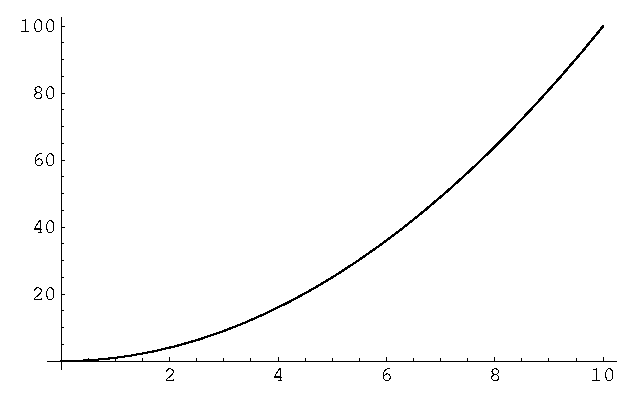
\includegraphics{images/plot.eps}
  \caption{%
    By default figures are not centered.
    This is a long caption to demonstrate that captions are single spaced.
  }
  \label{fi:not-centered}
\end{figure}

\Repeat{This is the second paragraph.}{10}

\begin{figure}[h]
  \centering
  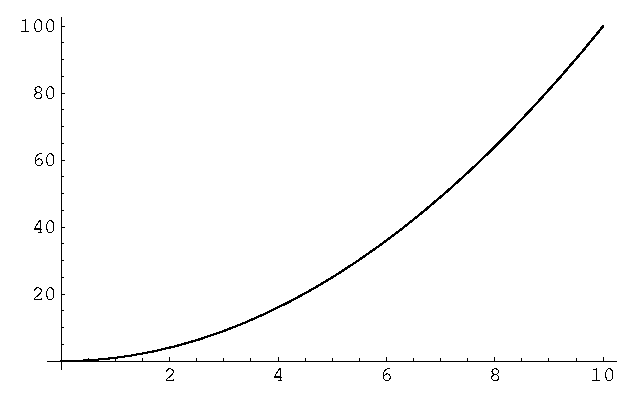
\includegraphics{images/plot.eps}
  \caption{Use {\tt \char'134centering\/} to center figures.}
  \label{fi:centered}
\end{figure}

\Repeat{This is the third paragraph.}{15}

\begin{figure}[h]
  \centering
  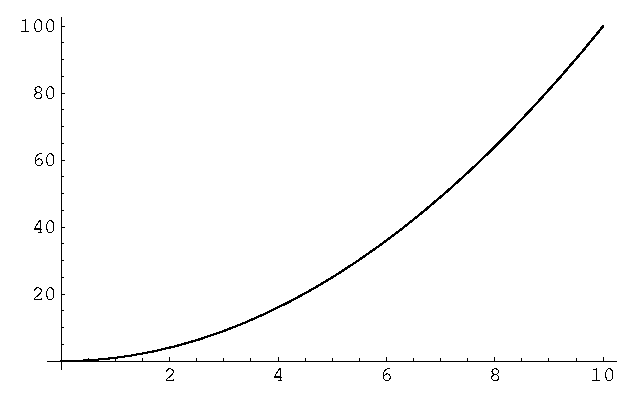
\includegraphics{images/plot.eps}
  \caption{This is another figuure.}
  \label{fi:another}
\end{figure}

\Repeat{This is the fourth paragraph.}{10}

\begin{figure}[h]
  \centering 
  \subfigure[First subcaption.]{\label{sf:two-parts-a}  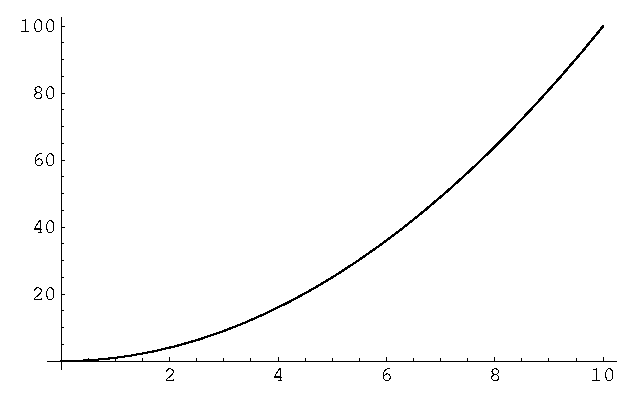
\includegraphics[width=0.3\textwidth]{images/plot.eps}}%
  \hskip 0.5truein
  \subfigure[Second subcaption.]{\label{sf:two-parts-b}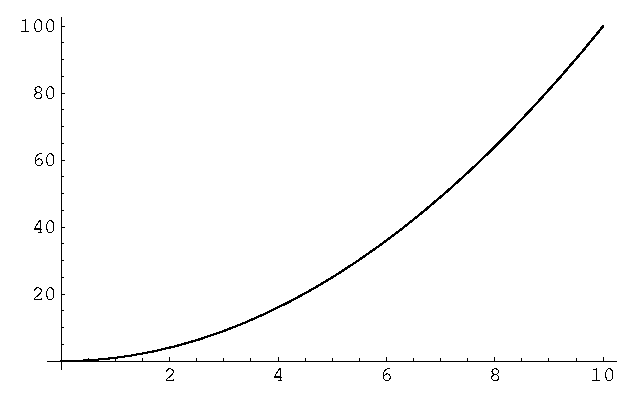
\includegraphics[width=0.3\textwidth]{images/plot.eps}}
  \caption{This figure has two parts.}
  \label{fi:two-parts}
\end{figure}

\Repeat{This is the fifth paragraph.}{10}

\begin{figure}[h]
  \centering
  \subfigure[First subcaption.]{\label{sf:four-parts-a}  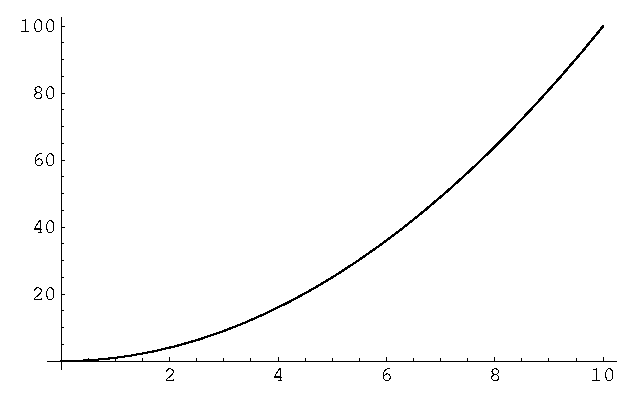
\includegraphics[width=0.3\textwidth]{images/plot.eps}}%
  \hskip 0.5truein
  \subfigure[Second subcaption.]{\label{sf:four-parts-b}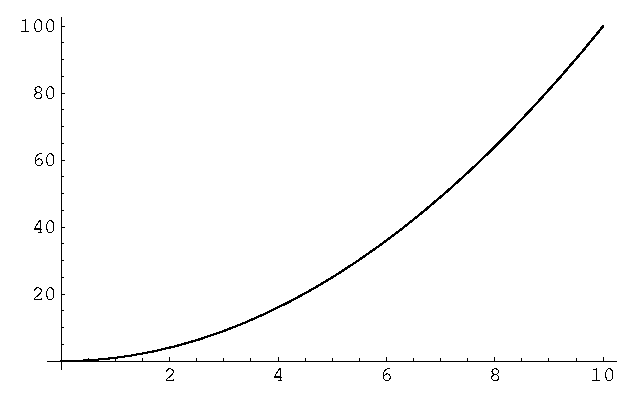
\includegraphics[width=0.3\textwidth]{images/plot.eps}}
  \subfigure[Third subcaption.]{\label{sf:four-parts-c}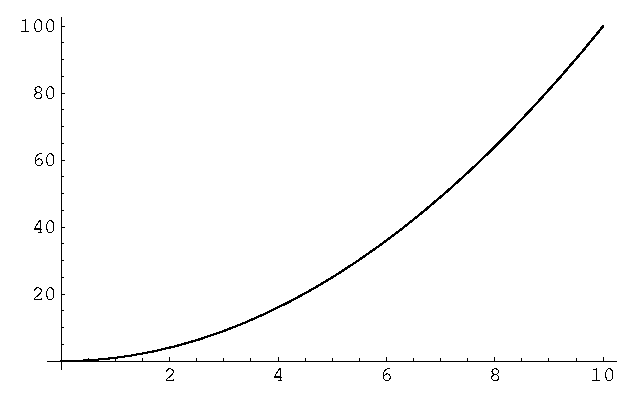
\includegraphics[width=0.3\textwidth]{images/plot.eps}}%
  \hskip 0.5truein
  \subfigure[Fourth subcaption.]{\label{sf:four-parts-d}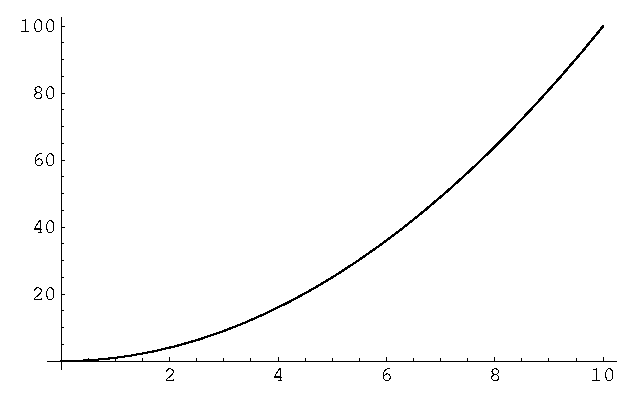
\includegraphics[width=0.3\textwidth]{images/plot.eps}}
  \caption{This figure has four parts.}
  \label{fi:four-parts}
\end{figure}

\Repeat{This is the sixth paragraph.}{10}

%%
%  THIS FILE DOES SOME UNUSUAL THINGS TO MAKE
%  IT EASIER TO DO DEMONSTRATIONS.  IT SHOULD
%  NOT BE USED AS AN EXAMPLE OF HOW TO PREPARE
%  A FILE.  SEE THE OUTPUT OF THIS FOR LATEX
%  INPUT AND OUTPUT EXAMPLES.
%




%
%  demo-mathematics.tex  2008-12-09  Mark Senn  http://engineering.purdue.edu/~mark
%

\chapter{Demonstrate Mathematics}

    % Use single spacing.
    \Baselinestretch{1}

    % You don't normally need this.
    \mbox{}

    \begin{verbatim}
% From _More Math Into LaTeX_, 4th Edition, page 152:
%     TeX uses $$ to open and close a displayed math environment.
%     In LaTeX, this may occassionally cause problems.  Don't do it.
\[
    E = mc^2
\]
    \end{verbatim}
% From _More Math Into LaTeX_, 4th Edition, page 152:
%     TeX uses $$ to open and close a displayed math environment.
%     In LaTeX, this may occassionally cause problems.  Don't do it.
\[
    E = mc^2
\]
    \vskip\baselineskip
    \hrule
    \vskip0.5\baselineskip
    \filbreak

    \begin{verbatim}
\begin{equation}
    E = mc^2
\end{equation}
    \end{verbatim}
\begin{equation}
    E = mc^2
\end{equation}
    \vskip\baselineskip
    \hrule
    \vskip0.5\baselineskip
    \filbreak

    \begin{verbatim}
% Mydefs.tex defines \be to be \begin{equation} and
% \ee to be \end{equation}.
\be
    E = mc^2
\ee
    \end{verbatim}
% Mydefs.tex defines \be to be \begin{equation} and
% \ee to be \end{equation}.
\be
    E = mc^2
\ee
    \vskip\baselineskip
    \hrule
    \vskip0.5\baselineskip
    \filbreak

    \begin{verbatim}
\be
    x = -\frac{b}{2a} \pm \frac{\sqrt{b^2 - 4ac}}{2a}
\ee
    \end{verbatim}
\be
    x = -\frac{b}{2a} \pm \frac{\sqrt{b^2 - 4ac}}{2a}
\ee
    \vskip\baselineskip
    \hrule
    \vskip0.5\baselineskip
    \filbreak

    \begin{verbatim}
% requires \usepackage{amsmath}; use align* for no equation number
\begin{align}
    a = {}& b + c\\
    x = {}& y + z
\end{align}
    \end{verbatim}
% requires \usepackage{amsmath}; use align* for no equation number
\begin{align}
    a = {}& b + c\\
    x = {}& y + z
\end{align}
    \vskip\baselineskip
    \hrule
    \vskip0.5\baselineskip
    \filbreak

    \begin{verbatim}
\[
    Z = \left(
        \begin{array}{cc}
            a& b\\
            c& d
        \end{array}
    \right)
\]
    \end{verbatim}
\[
    Z = \left(
        \begin{array}{cc}
            a& b\\
            c& d
        \end{array}
    \right)
\]
    \vskip\baselineskip
    \hrule
    \vskip0.5\baselineskip
    \filbreak

    \begin{verbatim}
\begin{equation}
    \begin{split}
        a = {}& b + c\\
            {}& + d + e
    \end{split}      
\end{equation}
    \end{verbatim}
\begin{equation}
    \begin{split}
        a = {}& b + c\\
            {}& + d + e
    \end{split}      
\end{equation}
    \vskip\baselineskip
    \hrule
    \vskip0.5\baselineskip
    \filbreak

    \begin{verbatim}
\be
    (\cos x)^2 + (\sin x)^2 = 1
\ee
    \end{verbatim}
\be
    (\cos x)^2 + (\sin x)^2 = 1
\ee
    \vskip\baselineskip
    \hrule
    \vskip0.5\baselineskip
    \filbreak

    \begin{verbatim}
If $X = \cos x$ and $Y = \sin x$ then $X^2 + Y^2 = 1$.
    \end{verbatim}
If $X = \cos x$ and $Y = \sin x$ then $X^2 + Y^2 = 1$.
    \vskip\baselineskip
    \hrule
    \vskip0.5\baselineskip
    \filbreak

%%
%  demo-multicols.tex  2007-03-19  Mark Senn  http://www.ecn.purdue.edu/~mark
%
%  Demonstrate multicols.
%
%  The multicols package must be loaded for this to work.
%  To load the multicols package put
%      \usepackage{multicols}
%  between the "\documentclass" and "\begin{document}" commands.
%

\chapter{Demonstrate Multicols}

% Put this amount of space between the columns.
\setlength{\columnsep}{0.5truein}

% Separate the columns with a vertical rule this wide.
\setlength{\columnseprule}{0.4pt}

\Repeat{This is one column.}{25}

\begin{multicols}{2}
\Repeat{This is two columns.}{25}
\end{multicols}

\begin{multicols}{3}
\Repeat{This is three columns.}{25}
\end{multicols}

\begin{multicols}{4}
\Repeat{This is four columns.}{25}
\end{multicols}

\begin{multicols}{5}
\Repeat{This is five columns.}{25}
\end{multicols}

%%
%  demo-tables.tex  2013-03-29  Mark Senn  http://engineering.purdue.edu/~mark
%
%  Demonstrate how to do tables.
%

\chapter{Demonstrate Tables}

% \newlength{\ta}
% \newlength{\tb}
% \newlength{\tc}
% 
% \settowidth{\ta}{\vbox{\hbox{Money}\hbox{Market}}}
% \settowidth{\tb}{\vbox{\hbox{Stocks}\hbox{and}\hbox{Bonds}}}
% \settowidth{\tc}{\vbox{\hbox{Money}\hbox{Market}\hbox{and}\hbox{Stocks}}}
% 
% {
%     \renewcommand{\baselinestretch}{1}
%     \begin{table}
%       \caption{%
%         \hfil Allocation of the IRA and Keogh Wealth\hfil\break
%         \mbox{}\hfil for Investors With or Without Brokerage Accounts\hfil
%       }
%       \label{tab:ira}
%       \begin{center}
%         \begin{tabular}%
%           {%
%             |%
%             c%
%             |%
%             >{\centering\hspace{0pt}}m{\the\ta}%  Money Market
%             |%
%             c%                                    Stocks 
%             |%
%             c%                                    Bonds
%             |%
%             c%                                    Diversified
%             |%
%             >{\centering\hspace{0pt}}m{\the\tb}%  Stocks and Bonds
%             |%
%             >{\centering\hspace{0pt}}m{\the\tc}%  Money Market and Stocks
%             |%
%             c%                                    Others
%             |%
%           }
%           \hline
%           IMP&
%             Money Market&
%             Stocks&
%             Bonds&
%             Diversified&
%             Stocks and Bonds&
%             Money Market and Stocks&
%             Others\tabularnewline
%           \hline
%           1& 14.19\%& 57.71\%& 12.21\%& 4.50\%& 7.36\%& 3.04\%& 0.99\%\tabularnewline \hline
%           2& 14.08\%& 58.18\%& 12.32\%& 4.44\%& 7.30\%& 2.80\%& 0.88\%\tabularnewline \hline
%           3 &14.26\%& 58.09\%& 12.27\%& 4.50\%& 7.19\%& 2.75\%& 0.94\%\tabularnewline \hline
%           4 &13.94\%& 58.11\%& 12.14\%& 4.78\%& 7.35\%& 2.68\%& 0.99\%\tabularnewline \hline
%           5 &13.92\%& 58.13\%& 11.93\%& 4.56\%& 7.60\%& 2.98\%& 0.88\%\tabularnewline \hline
%         \end{tabular}
%       \end{center}
%       This table presents the allocations of the wealth in the IRA
%       and Keogh accounts in various asset classes.
%       Results from each set of imputed data are presented here.
%       The first column lists the number of the imputations,
%       and rest of the columns lists various allocations.
%       Entrees under each asset class show the percentage of investors
%       who have most of their IRA
%       and Keogh wealth invested in that particular asset class.
%       The asset class Diversified
%       includes stocks,
%       bonds,
%       and money market investments.
%       The asset class Others
%       include investments in various life insurance products,
%       annuities,
%       real estate, etc.
%       \medskip
%     \footnotesize SOURCE: Survey of Consumer Finances,
%     2001,
%     Federal Reserve Board,
%     USA.\par
%   \end{table}
% }

Here is a really simple table.

% "h" means put table here---don't let it float to top or bottom of page
\begin{table}[h]
  \caption{American Presidents}
  \begin{center}
    \begin{tabular}{rl}
      \bf Number& \bf Name\\
      1& George Washington\\
      2& John Adams\\
      3& Thomas Jefferson\\
    \end{tabular}
  \end{center}
  \label{ta:American-Presidents}
\end{table}

There are 72.27 points per inch.
I like to put 2 points of vertical space between the heading
(Number Name)
and the first line
(1 George Washington)
of the table.

\begin{table}[h]
  \caption{American Presidents with 2pt vertical space after heading}
  \begin{center}
    \begin{tabular}{rl}
      \bf Number& \bf Name\\[2pt]  % put 2pt vertical space after this line
      1& George Washington\\
      2& John Adams\\
      3& Thomas Jefferson\\
    \end{tabular}
  \end{center}
  \label{ta:American-Presidents-with}
\end{table}

\LaTeX\ can print horizontal and vertical rules in tables.
I don't like the way this looks.

\begin{table}[h]
  \caption{American Presidents with horizontal and vertical lines}
  \begin{center}
    % "|" prints a vertical rule, "c" means center
    \begin{tabular}{|c|l|}
      % "\hline" prints a horizontal rule
      \hline
      \bf\#& \bf Name\\
      \hline
      1& George Washington\\
      \hline
      2& John Adams\\
      \hline
      3& Thomas Jefferson\\
      \hline
    \end{tabular}
  \end{center}
  \label{ta:American-Presidents-with}
\end{table}

\newpage

Here is a more complicated table.

\begin{table}[h]
  \caption{C Bitwise Operators}
  \begin{center}
    % "|" prints a vertical rule, "c" means center
    \begin{tabular}{cccc}
      \bf A& \bf B& \bf A$|$B& \bf A\&B\\[2pt]
      0& 0& 0& 0\\
      0& 1& 1& 0\\
      1& 0& 1& 0\\
      1& 1& 1& 1\\
    \end{tabular}
  \end{center}
  \label{ta:C-Bitwise}
\end{table}

You can use Plain \TeX's \verb+\halign+ command to make tables also.
If you can't do a complicated table using \LaTeX\ commands
you may want to try using Plain \TeX\ commands.
\LaTeX's table making commands use Plain \TeX\ commands.

\begin{table}[h]
  \caption{American Presidents using {\tt\char'134 halign}}
  \hbox to \textwidth{\hss\vbox{\halign{%
    \strut #&      % 0. \strut
    \hfil#\qquad&  % 1. Number
    #\hfil\cr      % 2. Name
    %
    & \bf Number& \bf Name\cr
    \noalign{\vskip 2pt}
    & 1& George Washington\cr
    & 2& John Adams\cr
    & 3& Thomas Jefferson\cr
  }}\hss}
  \label{ta:American-Presidents-using}
\end{table}

The next page shows how to do a table that is too long to fit on one page.

\newpage

% This is loosely based on page 106 of _A Guide to LaTeX_, third edition,
% by Helmut Kopka and Patrick W. Daly.
\begin{longtable}{|l|l|}
    \caption{State Abbreviations}\\
    \hline
    State& Abbreviation\\
    \hline
  \endfirsthead
    \caption[]{\emph{continued}}\\
    \hline
    State& Abbreviation\\
    \hline
  \endhead
    \hline
    \multicolumn{2}{r}{\emph{continued on next page}}
  \endfoot
    \hline
  \endlastfoot
  Alabama& AL\\
  Alaska& AK\\
% American Samoa& AS\\
  Arizona& AZ\\
  Arkansas& AR\\
% Armed Forces Europe& AE\\
% Armed Forces Pacific& AP\\
% Armed Forces the Americas& AA\\
  California& CA\\
  Colorado& CO\\
  Connecticut& CT\\
  Delaware& DE\\
% District of Columbia& DC\\
% Federated States of Micronesia& FM\\
  Florida& FL\\
  Georgia& GA\\
% Guam& GU\\
  Hawaii& HI\\
  Idaho& ID\\
  Illinois& IL\\
  Indiana& IN\\
  Iowa& IA\\
  Kansas& KS\\
  Kentucky& KY\\
  Louisiana& LA\\
  Maine& ME\\
% Marshall Islands& MH\\
  Maryland& MD\\
  Massachusetts& MA\\
  Michigan& MI\\
  Minnesota& MN\\
  Mississippi& MS\\
  Missouri& MO\\
  Montana& MT\\
  Nebraska& NE\\
  Nevada& NV\\
  New Hampshire& NH\\
  New Jersey& NJ\\
  New Mexico& NM\\
  New York& NY\\
  North Carolina& NC\\
  North Dakota& ND\\
% Northern Mariana Islands& MP\\
  Ohio& OH\\
  Oklahoma& OK\\
  Oregon& OR\\
  Pennsylvania& PA\\
% Puerto Rico& PR\\
  Rhode Island& RI\\
  South Carolina& SC\\
  South Dakota& SD\\
  Tennessee& TN\\
  Texas& TX\\
  Utah& UT\\
  Vermont& VT\\
% Virgin Islands& VI\\
  Virginia& VA\\
  Washington& WA\\
  West Virginia& WV\\
  Wisconsin& WI\\
  Wyoming& WY\\
\end{longtable}

\newcommand{\cbackslash}{\char'134}
\newcommand{\copencurly}{\char'173}
\newcommand{\cclosecurly}{\char'175}

\newlength{\twidth}
\newlength{\theight}

\setlength{\twidth}{\textwidth}
\setlength{\theight}{\textheight}

\begin{sidewaystable}
  % The following two lines compensate for what I think is a bug.
  \setlength{\textwidth}{\theight}
  \setlength{\textheight}{\twidth}
  \caption{%
    sidewaystable
    {\tt\cbackslash begin\copencurly tabular\cclosecurly\/}%
    \ldots
    {\tt\cbackslash end\copencurly tabular\cclosecurly\/}%
  }
  \begin{center}
    \begin{tabular}{rl}
      \bf Number& \bf Name\\[2pt]  % put 2pt vertical space after this line
      1& George Washington\\
      2& John Adams\\
      3& Thomas Jefferson\\
    \end{tabular}
  \end{center}
\end{sidewaystable}

\begin{sidewaystable}
  % The following two lines compensate for what I think is a bug.
  \setlength{\textwidth}{\theight}
  \setlength{\textheight}{\twidth}
  \caption{%
    sidewaystable
    {\tt\cbackslash halign\copencurly}\ldots{\tt\cclosecurly\/} table%
  }
  \hbox to \textwidth{\hss\vbox{\halign{%
    \strut #&      % 0. \strut
    \hfil#\qquad&  % 1. Number
    #\hfil\cr      % 2. Name
    %
    & \bf Number& \bf Name\cr
    \noalign{\vskip 2pt}
    & 1& George Washington\cr
    & 2& John Adams\cr
    & 3& Thomas Jefferson\cr
  }}\hss}
\end{sidewaystable}

%\newlength{\ta}
%\settowidth{\ta}{\vbox{\hbox{Money}\hbox{Market}}}
%\newlength{\tb}
%\settowidth{\tb}{\vbox{\hbox{Stocks}\hbox{and}\hbox{Bonds}}}
%\newlength{\tc}
%\settowidth{\tc}{\vbox{\hbox{Money}\hbox{Market}\hbox{and}\hbox{Stocks}}}
%
%  {\renewcommand{\baselinestretch}{1}
%\begin{table}
%  \caption{\hfil Allocation of the IRA and Keogh Wealth\hfil\break\mbox{}\hfil for Investors With or Without Brokerage Accounts\hfil}
%  \label{tab:ira}
%  \begin{center}
%    \begin{tabular}%
%      {%
%        |%
%        c%
%        |%
%        >{\centering\hspace{0pt}}m{\the\ta}%  Money Market
%        |%
%        c%                                    Stocks 
%        |%
%        c%                                    Bonds
%        |%
%        c%                                    Diversified
%        |%
%        >{\centering\hspace{0pt}}m{\the\tb}%  Stocks and Bonds
%        |%
%        >{\centering\hspace{0pt}}m{\the\tc}%  Money Market and Stocks
%        |%
%        c%                                    Others
%        |%
%      }
%      \hline
%      IMP&
%        Money Market&
%        Stocks&
%        Bonds&
%        Diversified&
%        Stocks and Bonds&
%        Money Market and Stocks&
%        Others\tabularnewline
%      \hline
%      1& 14.19\%& 57.71\%& 12.21\%& 4.50\%& 7.36\%& 3.04\%& 0.99\%\tabularnewline \hline
%      2& 14.08\%& 58.18\%& 12.32\%& 4.44\%& 7.30\%& 2.80\%& 0.88\%\tabularnewline \hline
%      3 &14.26\%& 58.09\%& 12.27\%& 4.50\%& 7.19\%& 2.75\%& 0.94\%\tabularnewline \hline
%      4 &13.94\%& 58.11\%& 12.14\%& 4.78\%& 7.35\%& 2.68\%& 0.99\%\tabularnewline \hline
%      5 &13.92\%& 58.13\%& 11.93\%& 4.56\%& 7.60\%& 2.98\%& 0.88\%\tabularnewline \hline
%    \end{tabular}
%  \end{center}
%  This table presents the allocations of the wealth in the IRA
%  and Keogh accounts in various asset classes.
%  Results from each set of imputed data are presented here.
%  The first column lists the number of the imputations,
%  and rest of the columns lists various allocations.
%  Entrees under each asset class show the percentage of investors
%  who have most of their IRA
%  and Keogh wealth invested in that particular asset class.
%  The asset class Diversified
%  includes stocks,
%  bonds,
%  and money market investments.
%  The asset class Others
%  include investments in various life insurance products,
%  annuities,
%  real estate, etc.
%  \medskip
%  \footnotesize SOURCE: Survey of Consumer Finances,
%  2001,
%  Federal Reserve Board,
%  USA.\par
%\end{table}
%  }


%%
%  demo-text.tex  2007-07-17  Mark Senn  http://engineering.purdue.edu/~mark
%

\chapter{Demonstrate Text}

% Use single spacing.
\Baselinestretch{1}

% You don't normally need this.
\mbox{}


%\vbox{
\begin{verbatim}
This is a sentence.
This is a sentence.
This is a sentence.
This is a sentence.
This is a sentence.

This is a sentence.
This is a sentence.
This is a sentence.
This is a sentence.
This is a sentence.
\end{verbatim}
This is a sentence.
This is a sentence.
This is a sentence.
This is a sentence.
This is a sentence.

This is a sentence.
This is a sentence.
This is a sentence.
This is a sentence.
This is a sentence.
\vskip\baselineskip
\hrule
%}
\vskip0.5\baselineskip
\filbreak

%\vbox{
\begin{verbatim}
From \verb+http://www.biblegateway.com/passage/?book_id=1&chapter=1&version=50+:

\begin{quote}
    1 In the beginning God created the heavens and the earth.
    2 The earth was without form,
    and void;
    and darkness was on the face of the deep.
    And the Spirit of God was hovering over the face of the waters.

    3 Then God said,``Let there be light'';
    and there was light.
    4 And God saw the light,
    that it was good;
    and God divided the light from the darkness.
    5 God called the light Day,
    and the darkness He called Night.
    So the evening and the morning were the first day. 
\end{quote}
\end{verbatim}
From \verb+http://www.biblegateway.com/passage/?book_id=1&chapter=1&version=50+:

\begin{quote}
    1 In the beginning God created the heavens and the earth.
    2 The earth was without form,
    and void;
    and darkness was on the face of the deep.
    And the Spirit of God was hovering over the face of the waters.

    3 Then God said,``Let there be light'';
    and there was light.
    4 And God saw the light,
    that it was good;
    and God divided the light from the darkness.
    5 God called the light Day,
    and the darkness He called Night.
    So the evening and the morning were the first day. 
\end{quote}
\vskip\baselineskip
\hrule
%}
\vskip0.5\baselineskip
\filbreak

%\vbox{
\begin{verbatim}
\begin{description}
    \item[apple]
        A red fruit.
    \item[banana]
        A yellow fruit.
        This sentence is to make the entry longer so you can see what happens.
        This sentence is to make the entry longer so you can see what happens.
    \item[cherry]
        A red friut.
\end{description}
\end{verbatim}
\begin{description}
    \item[apple]
        A red fruit.
    \item[banana]
        A yellow fruit.
        This sentence is to make the entry longer so you can see what happens.
        This sentence is to make the entry longer so you can see what happens.
    \item[cherry]
        A red friut.
\end{description}
\vskip\baselineskip
\hrule
%}
\vskip0.5\baselineskip
\filbreak

%\vbox{
\begin{verbatim}
\begin{enumerate}
    \item apple
    \item banana
        This sentence is to make the entry longer so you can see what happens.
        This sentence is to make the entry longer so you can see what happens.
    \item cherry
\end{enumerate}
\end{verbatim}
\begin{enumerate}
    \item apple
    \item banana
        This sentence is to make the entry longer so you can see what happens.
        This sentence is to make the entry longer so you can see what happens.
    \item cherry
\end{enumerate}
\vskip\baselineskip
\hrule
%}
\vskip0.5\baselineskip
\filbreak


%\vbox{
\begin{verbatim}
\begin{itemize}
    \item apple
    \item banana
        This sentence is to make the entry longer so you can see what happens.
        This sentence is to make the entry longer so you can see what happens.
    \item cherry
\end{itemize}
\end{verbatim}
\begin{itemize}
    \item apple
    \item banana
        This sentence is to make the entry longer so you can see what happens.
        This sentence is to make the entry longer so you can see what happens.
    \item cherry
\end{itemize}
\vskip\baselineskip
\hrule
%}
\vskip0.5\baselineskip
\filbreak


% Notes and footnotes are optional.
% Reference: TM 34.
% I have not implemented this yet.  Mark Senn 2002-06-03
%%\chapter{Notes}

\begin{itemize}
	\item Do we hash node's id in the commitment field of its data-item? NO
	\item Do we send the payload signature in case of Figure 5.4? YES
\end{itemize}

To do list:
\begin{itemize}
	% \item ch-3: signatures from 628; All PKI are not digital signatures capable.
	% \item ch-5: Clear goals of the protocol.
	% \item Review the writing.
	% \item ch-2: Add smooth transition to the security section.
	% \item ch-2: add more applications in section 2.1.
	% \item ch-4: change sign label
	% \item ch-4: Why SHIA does not have ID in their label? Why do you have ID? What benefits you get out of it?
	\item Cheating: Finish writing about detecting a cheater.
	\item ch-4: Image modifications. Update images with darker borders. Decrease width. Save word as pdf and then crop images
	\item Review the writing.

	\item 3. Discuss cheating, distributing off-path.  
	\item ch-6: Why don't you need signatures with off-path?
	\item ch-4: Advantages of signing the B's payload.

	\item ch-3: cite book for digital signatures

	\item ch-6: removing old signatures, and signing those again
	\item ch-6: equation for number of certificates needed in the network

\end{itemize}

% A vita is optional for masters theses
% and required for doctoral dissertations.
% Reference: TM 13.
% CHANGE NEXT LINE?
%%
%  vita.tex   2003.07.23  14:59:33   Mark Senn <mds@purdue.edu>
%
%  This is the vita for a simple, example thesis.
%
%  A vita is required only in a doctoral dissertation.
%

\begin{vita}
    [Put a brief autobiographical sketch here.]
\end{vita}


\end{document}

% LaTeX won't read after the \end{document} command.
% You can put notes to yourself or LaTeX input not
% ready for use here if you'd like.
